\documentclass[1p]{elsarticle_modified}
%\bibliographystyle{elsarticle-num}

%\usepackage[colorlinks]{hyperref}
%\usepackage{abbrmath_seonhwa} %\Abb, \Ascr, \Acal ,\Abf, \Afrak
\usepackage{amsfonts}
\usepackage{amssymb}
\usepackage{amsmath}
\usepackage{amsthm}
\usepackage{scalefnt}
\usepackage{amsbsy}
\usepackage{kotex}
\usepackage{caption}
\usepackage{subfig}
\usepackage{color}
\usepackage{graphicx}
\usepackage{xcolor} %% white, black, red, green, blue, cyan, magenta, yellow
\usepackage{float}
\usepackage{setspace}
\usepackage{hyperref}

\usepackage{tikz}
\usetikzlibrary{arrows}

\usepackage{multirow}
\usepackage{array} % fixed length table
\usepackage{hhline}

%%%%%%%%%%%%%%%%%%%%%
\makeatletter
\renewcommand*\env@matrix[1][\arraystretch]{%
	\edef\arraystretch{#1}%
	\hskip -\arraycolsep
	\let\@ifnextchar\new@ifnextchar
	\array{*\c@MaxMatrixCols c}}
\makeatother %https://tex.stackexchange.com/questions/14071/how-can-i-increase-the-line-spacing-in-a-matrix
%%%%%%%%%%%%%%%

\usepackage[normalem]{ulem}

\newcommand{\msout}[1]{\ifmmode\text{\sout{\ensuremath{#1}}}\else\sout{#1}\fi}
%SOURCE: \msout is \stkout macro in https://tex.stackexchange.com/questions/20609/strikeout-in-math-mode

\newcommand{\cancel}[1]{
	\ifmmode
	{\color{red}\msout{#1}}
	\else
	{\color{red}\sout{#1}}
	\fi
}

\newcommand{\add}[1]{
	{\color{blue}\uwave{#1}}
}

\newcommand{\replace}[2]{
	\ifmmode
	{\color{red}\msout{#1}}{\color{blue}\uwave{#2}}
	\else
	{\color{red}\sout{#1}}{\color{blue}\uwave{#2}}
	\fi
}

\newcommand{\Sol}{\mathcal{S}} %segment
\newcommand{\D}{D} %diagram
\newcommand{\A}{\mathcal{A}} %arc


%%%%%%%%%%%%%%%%%%%%%%%%%%%%%5 test

\def\sl{\operatorname{\textup{SL}}(2,\Cbb)}
\def\psl{\operatorname{\textup{PSL}}(2,\Cbb)}
\def\quan{\mkern 1mu \triangleright \mkern 1mu}

\theoremstyle{definition}
\newtheorem{thm}{Theorem}[section]
\newtheorem{prop}[thm]{Proposition}
\newtheorem{lem}[thm]{Lemma}
\newtheorem{ques}[thm]{Question}
\newtheorem{cor}[thm]{Corollary}
\newtheorem{defn}[thm]{Definition}
\newtheorem{exam}[thm]{Example}
\newtheorem{rmk}[thm]{Remark}
\newtheorem{alg}[thm]{Algorithm}

\newcommand{\I}{\sqrt{-1}}
\begin{document}

%\begin{frontmatter}
%
%\title{Boundary parabolic representations of knots up to 8 crossings}
%
%%% Group authors per affiliation:
%\author{Yunhi Cho} 
%\address{Department of Mathematics, University of Seoul, Seoul, Korea}
%\ead{yhcho@uos.ac.kr}
%
%
%\author{Seonhwa Kim} %\fnref{s_kim}}
%\address{Center for Geometry and Physics, Institute for Basic Science, Pohang, 37673, Korea}
%\ead{ryeona17@ibs.re.kr}
%
%\author{Hyuk Kim}
%\address{Department of Mathematical Sciences, Seoul National University, Seoul 08826, Korea}
%\ead{hyukkim@snu.ac.kr}
%
%\author{Seokbeom Yoon}
%\address{Department of Mathematical Sciences, Seoul National University, Seoul, 08826,  Korea}
%\ead{sbyoon15@snu.ac.kr}
%
%\begin{abstract}
%We find all boundary parabolic representation of knots up to 8 crossings.
%
%\end{abstract}
%\begin{keyword}
%    \MSC[2010] 57M25 
%\end{keyword}
%
%\end{frontmatter}

%\linenumbers
%\tableofcontents
%
\newcommand\colored[1]{\textcolor{white}{\rule[-0.35ex]{0.8em}{1.4ex}}\kern-0.8em\color{red} #1}%
%\newcommand\colored[1]{\textcolor{white}{ #1}\kern-2.17ex	\textcolor{white}{ #1}\kern-1.81ex	\textcolor{white}{ #1}\kern-2.15ex\color{red}#1	}

{\Large $\underline{12a_{1152}~(K12a_{1152})}$}

\setlength{\tabcolsep}{10pt}
\renewcommand{\arraystretch}{1.6}
\vspace{1cm}\begin{tabular}{m{100pt}>{\centering\arraybackslash}m{274pt}}
\multirow{5}{120pt}{
	\centering
	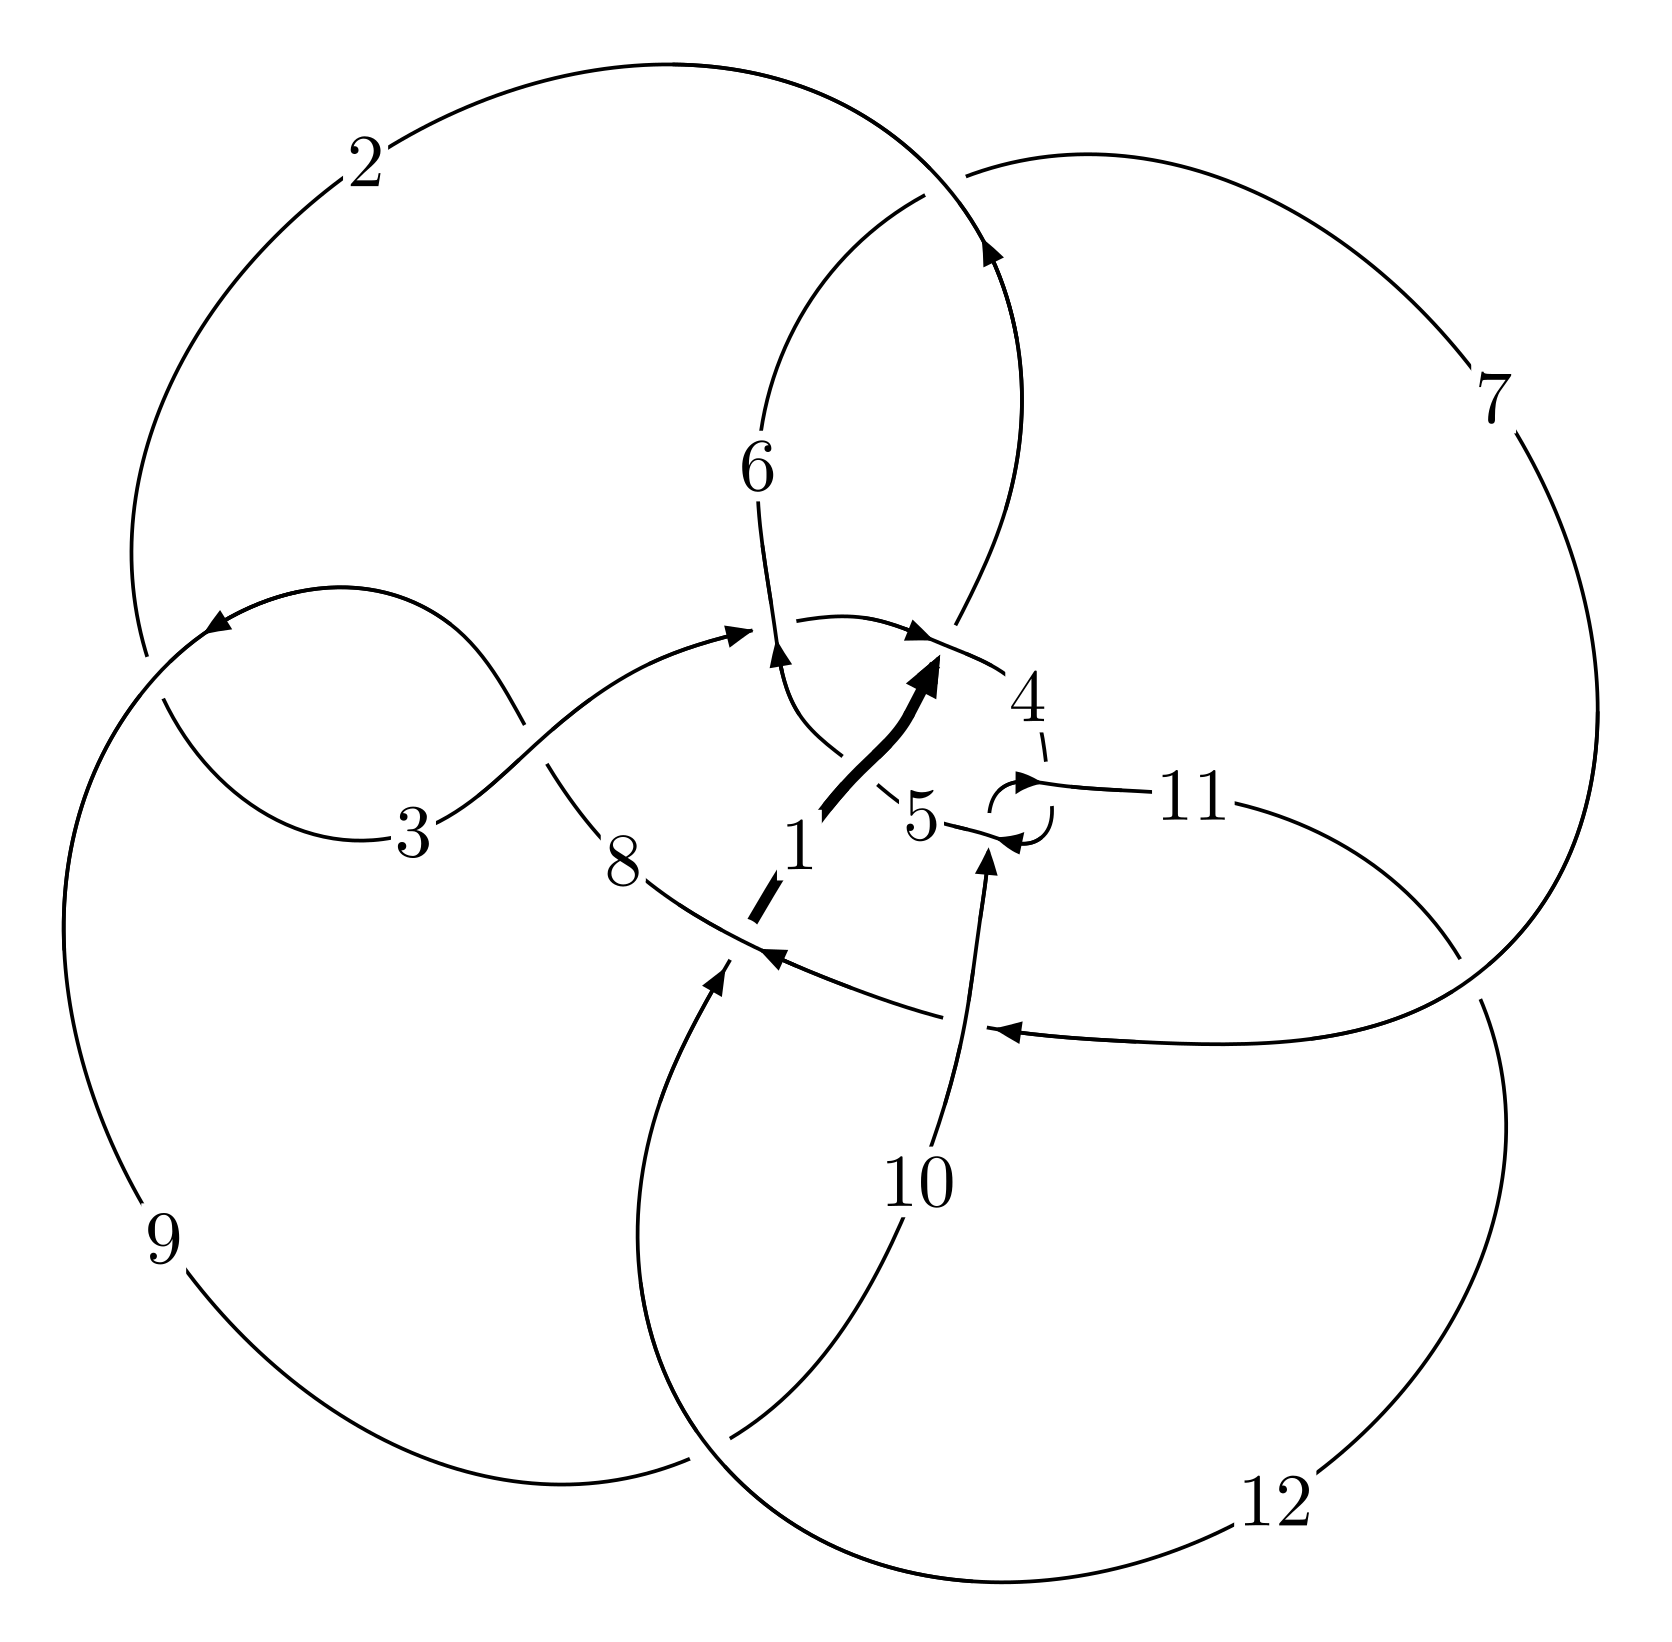
\includegraphics[width=112pt]{../../../GIT/diagram.site/Diagrams/png/1953_12a_1152.png}\\
\ \ \ A knot diagram\footnotemark}&
\allowdisplaybreaks
\textbf{Linearized knot diagam} \\
\cline{2-2}
 &
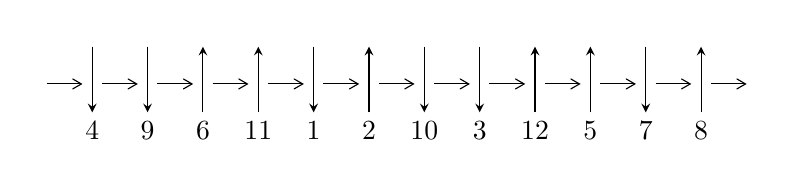
\begin{tikzpicture}[x=20pt, y=17pt]
	% nodes
	\node (C0) at (0, 0) {};
	\node (C1) at (1, 0) {};
	\node (C1U) at (1, +1) {};
	\node (C1D) at (1, -1) {4};

	\node (C2) at (2, 0) {};
	\node (C2U) at (2, +1) {};
	\node (C2D) at (2, -1) {9};

	\node (C3) at (3, 0) {};
	\node (C3U) at (3, +1) {};
	\node (C3D) at (3, -1) {6};

	\node (C4) at (4, 0) {};
	\node (C4U) at (4, +1) {};
	\node (C4D) at (4, -1) {11};

	\node (C5) at (5, 0) {};
	\node (C5U) at (5, +1) {};
	\node (C5D) at (5, -1) {1};

	\node (C6) at (6, 0) {};
	\node (C6U) at (6, +1) {};
	\node (C6D) at (6, -1) {2};

	\node (C7) at (7, 0) {};
	\node (C7U) at (7, +1) {};
	\node (C7D) at (7, -1) {10};

	\node (C8) at (8, 0) {};
	\node (C8U) at (8, +1) {};
	\node (C8D) at (8, -1) {3};

	\node (C9) at (9, 0) {};
	\node (C9U) at (9, +1) {};
	\node (C9D) at (9, -1) {12};

	\node (C10) at (10, 0) {};
	\node (C10U) at (10, +1) {};
	\node (C10D) at (10, -1) {5};

	\node (C11) at (11, 0) {};
	\node (C11U) at (11, +1) {};
	\node (C11D) at (11, -1) {7};

	\node (C12) at (12, 0) {};
	\node (C12U) at (12, +1) {};
	\node (C12D) at (12, -1) {8};
	\node (C13) at (13, 0) {};

	% arrows
	\draw[->,>={angle 60}]
	(C0) edge (C1) (C1) edge (C2) (C2) edge (C3) (C3) edge (C4) (C4) edge (C5) (C5) edge (C6) (C6) edge (C7) (C7) edge (C8) (C8) edge (C9) (C9) edge (C10) (C10) edge (C11) (C11) edge (C12) (C12) edge (C13) ;	\draw[->,>=stealth]
	(C1U) edge (C1D) (C2U) edge (C2D) (C3D) edge (C3U) (C4D) edge (C4U) (C5U) edge (C5D) (C6D) edge (C6U) (C7U) edge (C7D) (C8U) edge (C8D) (C9D) edge (C9U) (C10D) edge (C10U) (C11U) edge (C11D) (C12D) edge (C12U) ;
	\end{tikzpicture} \\
\hhline{~~} \\& 
\textbf{Solving Sequence} \\ \cline{2-2} 
 &
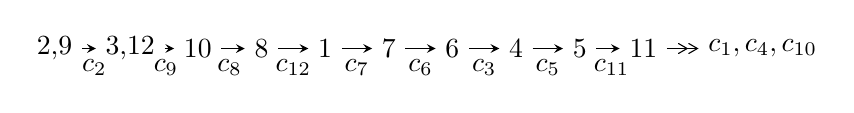
\begin{tikzpicture}[x=23pt, y=7pt]
	% node
	\node (A0) at (-1/8, 0) {2,9};
	\node (A1) at (17/16, 0) {3,12};
	\node (A2) at (17/8, 0) {10};
	\node (A3) at (25/8, 0) {8};
	\node (A4) at (33/8, 0) {1};
	\node (A5) at (41/8, 0) {7};
	\node (A6) at (49/8, 0) {6};
	\node (A7) at (57/8, 0) {4};
	\node (A8) at (65/8, 0) {5};
	\node (A9) at (73/8, 0) {11};
	\node (C1) at (1/2, -1) {$c_{2}$};
	\node (C2) at (13/8, -1) {$c_{9}$};
	\node (C3) at (21/8, -1) {$c_{8}$};
	\node (C4) at (29/8, -1) {$c_{12}$};
	\node (C5) at (37/8, -1) {$c_{7}$};
	\node (C6) at (45/8, -1) {$c_{6}$};
	\node (C7) at (53/8, -1) {$c_{3}$};
	\node (C8) at (61/8, -1) {$c_{5}$};
	\node (C9) at (69/8, -1) {$c_{11}$};
	\node (A10) at (11, 0) {$c_{1},c_{4},c_{10}$};

	% edge
	\draw[->,>=stealth]	
	(A0) edge (A1) (A1) edge (A2) (A2) edge (A3) (A3) edge (A4) (A4) edge (A5) (A5) edge (A6) (A6) edge (A7) (A7) edge (A8) (A8) edge (A9) ;
	\draw[->>,>={angle 60}]	
	(A9) edge (A10);
\end{tikzpicture} \\ 

\end{tabular} \\

\footnotetext{
The image of knot diagram is generated by the software ``\textbf{Draw programme}" developed by Andrew Bartholomew(\url{http://www.layer8.co.uk/maths/draw/index.htm\#Running-draw}), where we modified some parts for our purpose(\url{https://github.com/CATsTAILs/LinksPainter}).
}\phantom \\ \newline 
\centering \textbf{Ideals for irreducible components\footnotemark of $X_{\text{par}}$} 
 
\begin{align*}
I^u_{1}&=\langle 
-5.18767\times10^{139} u^{59}+6.91498\times10^{140} u^{58}+\cdots+5.70794\times10^{142} b-4.09699\times10^{143},\\
\phantom{I^u_{1}}&\phantom{= \langle  }-1.69716\times10^{143} u^{59}+7.21637\times10^{143} u^{58}+\cdots+5.53670\times10^{144} a+2.20134\times10^{145},\\
\phantom{I^u_{1}}&\phantom{= \langle  }u^{60}-5 u^{59}+\cdots+1080 u-388\rangle \\
I^u_{2}&=\langle 
1.80510\times10^{155} a u^{81}-1.97549\times10^{154} u^{81}+\cdots+1.30403\times10^{156} a+5.44654\times10^{156},\\
\phantom{I^u_{2}}&\phantom{= \langle  }3.60091\times10^{156} a u^{81}+2.53871\times10^{156} u^{81}+\cdots+1.70950\times10^{158} a-1.03794\times10^{158},\\
\phantom{I^u_{2}}&\phantom{= \langle  }u^{82}+2 u^{81}+\cdots+3 u+17\rangle \\
I^u_{3}&=\langle 
-9.59808\times10^{21} u^{51}+4.27636\times10^{20} u^{50}+\cdots+1.61406\times10^{20} b+5.52488\times10^{21},\\
\phantom{I^u_{3}}&\phantom{= \langle  }-4.99289\times10^{18} u^{51}-9.77290\times10^{20} u^{50}+\cdots+1.61406\times10^{20} a-5.20434\times10^{21},\\
\phantom{I^u_{3}}&\phantom{= \langle  }u^{52}+12 u^{50}+\cdots+16 u^2+1\rangle \\
I^u_{4}&=\langle 
b- u-2,\;a- u,\;u^2+u+1\rangle \\
I^u_{5}&=\langle 
b+3 u-2,\;a+u,\;u^2- u+1\rangle \\
I^u_{6}&=\langle 
-2 u^3-3 u^2+3 b-3 u-1,\;4 u^3+6 u^2+3 a+6 u-1,\;u^4+2 u^3+3 u^2+2 u+1\rangle \\
I^u_{7}&=\langle 
4 u^3-6 u^2+3 b+9 u-5,\;2 u^3-3 u^2+a+4 u-1,\;u^4-2 u^3+3 u^2-2 u+1\rangle \\
I^u_{8}&=\langle 
b- u,\;a,\;u^2+u+1\rangle \\
I^u_{9}&=\langle 
b+u+1,\;a-1,\;u^2+u+1\rangle \\
\\
I^v_{1}&=\langle 
a,\;b^2- b+1,\;v+1\rangle \\
\end{align*}
\raggedright * 10 irreducible components of $\dim_{\mathbb{C}}=0$, with total 294 representations.\\
\footnotetext{All coefficients of polynomials are rational numbers. But the coefficients are sometimes approximated in decimal forms when there is not enough margin.}
\newpage
\renewcommand{\arraystretch}{1}
\centering \section*{I. $I^u_{1}= \langle -5.19\times10^{139} u^{59}+6.91\times10^{140} u^{58}+\cdots+5.71\times10^{142} b-4.10\times10^{143},\;-1.70\times10^{143} u^{59}+7.22\times10^{143} u^{58}+\cdots+5.54\times10^{144} a+2.20\times10^{145},\;u^{60}-5 u^{59}+\cdots+1080 u-388 \rangle$}
\flushleft \textbf{(i) Arc colorings}\\
\begin{tabular}{m{7pt} m{180pt} m{7pt} m{180pt} }
\flushright $a_{2}=$&$\begin{pmatrix}1\\0\end{pmatrix}$ \\
\flushright $a_{9}=$&$\begin{pmatrix}0\\u\end{pmatrix}$ \\
\flushright $a_{3}=$&$\begin{pmatrix}1\\u^2\end{pmatrix}$ \\
\flushright $a_{12}=$&$\begin{pmatrix}0.0306529 u^{59}-0.130337 u^{58}+\cdots-4.49260 u-3.97590\\0.000908851 u^{59}-0.0121147 u^{58}+\cdots-16.7204 u+7.17771\end{pmatrix}$ \\
\flushright $a_{10}=$&$\begin{pmatrix}-0.0291167 u^{59}+0.173061 u^{58}+\cdots+55.3140 u-16.6802\\-0.00711532 u^{59}+0.0485395 u^{58}+\cdots+22.8821 u-6.56340\end{pmatrix}$ \\
\flushright $a_{8}=$&$\begin{pmatrix}u\\u^3+u\end{pmatrix}$ \\
\flushright $a_{1}=$&$\begin{pmatrix}0.0414282 u^{59}-0.173898 u^{58}+\cdots-0.281038 u-8.05200\\0.00626255 u^{59}-0.0383628 u^{58}+\cdots-19.4695 u+7.10429\end{pmatrix}$ \\
\flushright $a_{7}=$&$\begin{pmatrix}0.0149334 u^{59}-0.0977080 u^{58}+\cdots-41.4306 u+15.7688\\0.0105054 u^{59}-0.0633023 u^{58}+\cdots-22.1161 u+7.13426\end{pmatrix}$ \\
\flushright $a_{6}=$&$\begin{pmatrix}0.00442802 u^{59}-0.0344057 u^{58}+\cdots-19.3145 u+8.63453\\0.0105054 u^{59}-0.0633023 u^{58}+\cdots-22.1161 u+7.13426\end{pmatrix}$ \\
\flushright $a_{4}=$&$\begin{pmatrix}-0.0443936 u^{59}+0.179043 u^{58}+\cdots-14.6753 u+15.9101\\-0.00517660 u^{59}+0.0333438 u^{58}+\cdots+14.3685 u-5.35765\end{pmatrix}$ \\
\flushright $a_{5}=$&$\begin{pmatrix}0.0422065 u^{59}-0.254284 u^{58}+\cdots-87.5145 u+30.4184\\-0.00436150 u^{59}-0.00212137 u^{58}+\cdots-19.7603 u+10.9710\end{pmatrix}$ \\
\flushright $a_{11}=$&$\begin{pmatrix}0.0715267 u^{59}-0.304662 u^{58}+\cdots-20.9895 u-5.59872\\0.0150082 u^{59}-0.0735745 u^{58}+\cdots-14.2922 u+4.17681\end{pmatrix}$\\&\end{tabular}
\flushleft \textbf{(ii) Obstruction class $= -1$}\\~\\
\flushleft \textbf{(iii) Cusp Shapes $= 0.0862410 u^{59}-0.304241 u^{58}+\cdots+50.6490 u-39.3628$}\\~\\
\newpage\renewcommand{\arraystretch}{1}
\flushleft \textbf{(iv) u-Polynomials at the component}\newline \\
\begin{tabular}{m{50pt}|m{274pt}}
Crossings & \hspace{64pt}u-Polynomials at each crossing \\
\hline $$\begin{aligned}c_{1},c_{7}\end{aligned}$$&$\begin{aligned}
&u^{60}-3 u^{59}+\cdots-8 u+1
\end{aligned}$\\
\hline $$\begin{aligned}c_{2},c_{8}\end{aligned}$$&$\begin{aligned}
&u^{60}-5 u^{59}+\cdots+1080 u-388
\end{aligned}$\\
\hline $$\begin{aligned}c_{3},c_{9}\end{aligned}$$&$\begin{aligned}
&u^{60}+3 u^{59}+\cdots+8 u+1
\end{aligned}$\\
\hline $$\begin{aligned}c_{4},c_{10}\end{aligned}$$&$\begin{aligned}
&u^{60}+5 u^{59}+\cdots-1080 u-388
\end{aligned}$\\
\hline $$\begin{aligned}c_{5},c_{11}\end{aligned}$$&$\begin{aligned}
&u^{60}+u^{59}+\cdots+16 u+1
\end{aligned}$\\
\hline $$\begin{aligned}c_{6},c_{12}\end{aligned}$$&$\begin{aligned}
&u^{60}- u^{59}+\cdots-16 u+1
\end{aligned}$\\
\hline
\end{tabular}\\~\\
\newpage\renewcommand{\arraystretch}{1}
\flushleft \textbf{(v) Riley Polynomials at the component}\newline \\
\begin{tabular}{m{50pt}|m{274pt}}
Crossings & \hspace{64pt}Riley Polynomials at each crossing \\
\hline $$\begin{aligned}c_{1},c_{3},c_{7}\\c_{9}\end{aligned}$$&$\begin{aligned}
&y^{60}-19 y^{59}+\cdots+260 y^2+1
\end{aligned}$\\
\hline $$\begin{aligned}c_{2},c_{4},c_{8}\\c_{10}\end{aligned}$$&$\begin{aligned}
&y^{60}+25 y^{59}+\cdots-621648 y+150544
\end{aligned}$\\
\hline $$\begin{aligned}c_{5},c_{6},c_{11}\\c_{12}\end{aligned}$$&$\begin{aligned}
&y^{60}-5 y^{59}+\cdots-124 y+1
\end{aligned}$\\
\hline
\end{tabular}\\~\\
\newpage\flushleft \textbf{(vi) Complex Volumes and Cusp Shapes}
$$\begin{array}{c|c|c}  
\text{Solutions to }I^u_{1}& \I (\text{vol} + \sqrt{-1}CS) & \text{Cusp shape}\\
 \hline 
\begin{aligned}
u &= \phantom{-}0.171441 + 0.980559 I \\
a &= \phantom{-}0.47348 + 1.49828 I \\
b &= -0.511578 + 0.392997 I\end{aligned}
 & -0.52610 + 2.40940 I & -6.07207 - 1.80479 I \\ \hline\begin{aligned}
u &= \phantom{-}0.171441 - 0.980559 I \\
a &= \phantom{-}0.47348 - 1.49828 I \\
b &= -0.511578 - 0.392997 I\end{aligned}
 & -0.52610 - 2.40940 I & -6.07207 + 1.80479 I \\ \hline\begin{aligned}
u &= \phantom{-}0.558795 + 0.812413 I \\
a &= \phantom{-}0.190007 - 0.772991 I \\
b &= \phantom{-}1.32190 - 0.62082 I\end{aligned}
 & \phantom{-}2.92685 - 2.53562 I & \phantom{-}7.77144 + 4.11547 I \\ \hline\begin{aligned}
u &= \phantom{-}0.558795 - 0.812413 I \\
a &= \phantom{-}0.190007 + 0.772991 I \\
b &= \phantom{-}1.32190 + 0.62082 I\end{aligned}
 & \phantom{-}2.92685 + 2.53562 I & \phantom{-}7.77144 - 4.11547 I \\ \hline\begin{aligned}
u &= \phantom{-}0.387995 + 0.880914 I \\
a &= \phantom{-}0.696357 - 1.223310 I \\
b &= \phantom{-}0.137839 - 0.769925 I\end{aligned}
 & \phantom{-}4.19283 - 1.62322 I & \phantom{-}9.54675 + 5.56587 I \\ \hline\begin{aligned}
u &= \phantom{-}0.387995 - 0.880914 I \\
a &= \phantom{-}0.696357 + 1.223310 I \\
b &= \phantom{-}0.137839 + 0.769925 I\end{aligned}
 & \phantom{-}4.19283 + 1.62322 I & \phantom{-}9.54675 - 5.56587 I \\ \hline\begin{aligned}
u &= -0.325924 + 1.003870 I \\
a &= \phantom{-}0.472335 + 0.390385 I \\
b &= -0.264203 + 0.121523 I\end{aligned}
 & \phantom{-0.000000 -}2.32702 I & \phantom{-0.000000 } 0. - 2.41446 I \\ \hline\begin{aligned}
u &= -0.325924 - 1.003870 I \\
a &= \phantom{-}0.472335 - 0.390385 I \\
b &= -0.264203 - 0.121523 I\end{aligned}
 & \phantom{-0.000000 } -2.32702 I & \phantom{-0.000000 -}0. + 2.41446 I \\ \hline\begin{aligned}
u &= -0.451519 + 0.956785 I \\
a &= \phantom{-}0.126006 + 0.783615 I \\
b &= \phantom{-}1.29360 + 1.08825 I\end{aligned}
 & \phantom{-}1.50162 + 6.66973 I & \phantom{-}6.52482 - 9.31381 I \\ \hline\begin{aligned}
u &= -0.451519 - 0.956785 I \\
a &= \phantom{-}0.126006 - 0.783615 I \\
b &= \phantom{-}1.29360 - 1.08825 I\end{aligned}
 & \phantom{-}1.50162 - 6.66973 I & \phantom{-}6.52482 + 9.31381 I\\
 \hline 
 \end{array}$$\newpage$$\begin{array}{c|c|c}  
\text{Solutions to }I^u_{1}& \I (\text{vol} + \sqrt{-1}CS) & \text{Cusp shape}\\
 \hline 
\begin{aligned}
u &= -0.405466 + 1.042930 I \\
a &= \phantom{-}0.300272 + 1.091020 I \\
b &= \phantom{-}0.575186 + 0.966227 I\end{aligned}
 & \phantom{-}1.77104 - 0.45619 I & \phantom{-}4.17621 + 0. I\phantom{ +0.000000I} \\ \hline\begin{aligned}
u &= -0.405466 - 1.042930 I \\
a &= \phantom{-}0.300272 - 1.091020 I \\
b &= \phantom{-}0.575186 - 0.966227 I\end{aligned}
 & \phantom{-}1.77104 + 0.45619 I & \phantom{-}4.17621 + 0. I\phantom{ +0.000000I} \\ \hline\begin{aligned}
u &= \phantom{-}1.058290 + 0.365526 I \\
a &= -1.030290 - 0.473394 I \\
b &= -0.97651 - 1.14607 I\end{aligned}
 & -7.37408 + 4.86636 I & -7.60593 - 5.88900 I \\ \hline\begin{aligned}
u &= \phantom{-}1.058290 - 0.365526 I \\
a &= -1.030290 + 0.473394 I \\
b &= -0.97651 + 1.14607 I\end{aligned}
 & -7.37408 - 4.86636 I & -7.60593 + 5.88900 I \\ \hline\begin{aligned}
u &= -1.13290\phantom{ +0.000000I} \\
a &= -0.870261\phantom{ +0.000000I} \\
b &= -1.73957\phantom{ +0.000000I}\end{aligned}
 & -0.677721\phantom{ +0.000000I} & -12.9010\phantom{ +0.000000I} \\ \hline\begin{aligned}
u &= \phantom{-}0.183453 + 0.841795 I \\
a &= -2.34687 + 0.35556 I \\
b &= -0.221990 - 0.196071 I\end{aligned}
 & -0.95944 - 4.24881 I & -12.3767 + 15.9835 I \\ \hline\begin{aligned}
u &= \phantom{-}0.183453 - 0.841795 I \\
a &= -2.34687 - 0.35556 I \\
b &= -0.221990 + 0.196071 I\end{aligned}
 & -0.95944 + 4.24881 I & -12.3767 - 15.9835 I \\ \hline\begin{aligned}
u &= \phantom{-}0.485164 + 1.033450 I \\
a &= -0.436484 - 0.472405 I \\
b &= \phantom{-}0.50964 - 1.98747 I\end{aligned}
 & -1.50162 - 6.66973 I & -6.52482 + 9.31381 I \\ \hline\begin{aligned}
u &= \phantom{-}0.485164 - 1.033450 I \\
a &= -0.436484 + 0.472405 I \\
b &= \phantom{-}0.50964 + 1.98747 I\end{aligned}
 & -1.50162 + 6.66973 I & -6.52482 - 9.31381 I \\ \hline\begin{aligned}
u &= -0.693664 + 0.378260 I \\
a &= \phantom{-}0.313816 - 0.578350 I \\
b &= -0.732368 - 0.379929 I\end{aligned}
 & -1.64774 + 0.88135 I & -5.13712 - 2.80459 I\\
 \hline 
 \end{array}$$\newpage$$\begin{array}{c|c|c}  
\text{Solutions to }I^u_{1}& \I (\text{vol} + \sqrt{-1}CS) & \text{Cusp shape}\\
 \hline 
\begin{aligned}
u &= -0.693664 - 0.378260 I \\
a &= \phantom{-}0.313816 + 0.578350 I \\
b &= -0.732368 + 0.379929 I\end{aligned}
 & -1.64774 - 0.88135 I & -5.13712 + 2.80459 I \\ \hline\begin{aligned}
u &= \phantom{-}1.168760 + 0.338858 I \\
a &= -0.072999 + 0.185626 I \\
b &= -0.917703 + 0.097618 I\end{aligned}
 & -5.39058 - 4.68678 I & \phantom{-0.000000 } 0 \\ \hline\begin{aligned}
u &= \phantom{-}1.168760 - 0.338858 I \\
a &= -0.072999 - 0.185626 I \\
b &= -0.917703 - 0.097618 I\end{aligned}
 & -5.39058 + 4.68678 I & \phantom{-0.000000 } 0 \\ \hline\begin{aligned}
u &= \phantom{-}0.531474 + 0.568901 I \\
a &= \phantom{-}0.968713 + 0.737512 I \\
b &= -1.10882 + 1.28934 I\end{aligned}
 & -2.92685 + 2.53562 I & -7.77144 - 4.11547 I \\ \hline\begin{aligned}
u &= \phantom{-}0.531474 - 0.568901 I \\
a &= \phantom{-}0.968713 - 0.737512 I \\
b &= -1.10882 - 1.28934 I\end{aligned}
 & -2.92685 - 2.53562 I & -7.77144 + 4.11547 I \\ \hline\begin{aligned}
u &= -1.165740 + 0.366483 I \\
a &= -1.038980 + 0.534131 I \\
b &= -0.85758 + 1.68385 I\end{aligned}
 & \phantom{-0.000000 } -9.35734 I & \phantom{-0.000000 } 0 \\ \hline\begin{aligned}
u &= -1.165740 - 0.366483 I \\
a &= -1.038980 - 0.534131 I \\
b &= -0.85758 - 1.68385 I\end{aligned}
 & \phantom{-0.000000 -}9.35734 I & \phantom{-0.000000 } 0 \\ \hline\begin{aligned}
u &= \phantom{-}0.418269 + 1.150070 I \\
a &= -0.197115 - 0.307278 I \\
b &= -0.32483 - 1.53729 I\end{aligned}
 & -1.77104 - 0.45619 I & \phantom{-0.000000 } 0 \\ \hline\begin{aligned}
u &= \phantom{-}0.418269 - 1.150070 I \\
a &= -0.197115 + 0.307278 I \\
b &= -0.32483 + 1.53729 I\end{aligned}
 & -1.77104 + 0.45619 I & \phantom{-0.000000 } 0 \\ \hline\begin{aligned}
u &= -0.499563 + 1.124770 I \\
a &= -0.175796 + 0.500266 I \\
b &= \phantom{-}0.320548 + 1.310060 I\end{aligned}
 & \phantom{-}0.62611 + 3.69051 I & \phantom{-0.000000 } 0\\
 \hline 
 \end{array}$$\newpage$$\begin{array}{c|c|c}  
\text{Solutions to }I^u_{1}& \I (\text{vol} + \sqrt{-1}CS) & \text{Cusp shape}\\
 \hline 
\begin{aligned}
u &= -0.499563 - 1.124770 I \\
a &= -0.175796 - 0.500266 I \\
b &= \phantom{-}0.320548 - 1.310060 I\end{aligned}
 & \phantom{-}0.62611 - 3.69051 I & \phantom{-0.000000 } 0 \\ \hline\begin{aligned}
u &= \phantom{-}1.193310 + 0.369826 I \\
a &= -0.992840 - 0.546634 I \\
b &= -0.67757 - 1.65324 I\end{aligned}
 & -2.9032 + 15.8984 I & \phantom{-0.000000 } 0 \\ \hline\begin{aligned}
u &= \phantom{-}1.193310 - 0.369826 I \\
a &= -0.992840 + 0.546634 I \\
b &= -0.67757 + 1.65324 I\end{aligned}
 & -2.9032 - 15.8984 I & \phantom{-0.000000 } 0 \\ \hline\begin{aligned}
u &= \phantom{-}0.076532 + 0.729921 I \\
a &= \phantom{-}1.110150 + 0.160313 I \\
b &= -2.61620 + 0.41046 I\end{aligned}
 & -4.19283 - 1.62322 I & -9.54675 + 5.56587 I \\ \hline\begin{aligned}
u &= \phantom{-}0.076532 - 0.729921 I \\
a &= \phantom{-}1.110150 - 0.160313 I \\
b &= -2.61620 - 0.41046 I\end{aligned}
 & -4.19283 + 1.62322 I & -9.54675 - 5.56587 I \\ \hline\begin{aligned}
u &= \phantom{-}0.426858 + 1.216580 I \\
a &= -0.177926 - 1.247300 I \\
b &= \phantom{-}1.34612 - 0.61746 I\end{aligned}
 & \phantom{-}5.39058 - 4.68678 I & \phantom{-0.000000 } 0 \\ \hline\begin{aligned}
u &= \phantom{-}0.426858 - 1.216580 I \\
a &= -0.177926 + 1.247300 I \\
b &= \phantom{-}1.34612 + 0.61746 I\end{aligned}
 & \phantom{-}5.39058 + 4.68678 I & \phantom{-0.000000 } 0 \\ \hline\begin{aligned}
u &= \phantom{-}1.30496\phantom{ +0.000000I} \\
a &= \phantom{-}0.771561\phantom{ +0.000000I} \\
b &= \phantom{-}1.53977\phantom{ +0.000000I}\end{aligned}
 & \phantom{-}0.677721\phantom{ +0.000000I} & \phantom{-0.000000 } 0 \\ \hline\begin{aligned}
u &= -0.419010 + 1.272320 I \\
a &= \phantom{-}0.33802 - 1.40935 I \\
b &= -1.55921 - 0.25601 I\end{aligned}
 & \phantom{-}3.80470 + 5.01319 I & \phantom{-0.000000 } 0 \\ \hline\begin{aligned}
u &= -0.419010 - 1.272320 I \\
a &= \phantom{-}0.33802 + 1.40935 I \\
b &= -1.55921 + 0.25601 I\end{aligned}
 & \phantom{-}3.80470 - 5.01319 I & \phantom{-0.000000 } 0\\
 \hline 
 \end{array}$$\newpage$$\begin{array}{c|c|c}  
\text{Solutions to }I^u_{1}& \I (\text{vol} + \sqrt{-1}CS) & \text{Cusp shape}\\
 \hline 
\begin{aligned}
u &= \phantom{-}0.638473 + 1.214620 I \\
a &= \phantom{-}0.318696 + 1.236200 I \\
b &= -1.62056 + 1.22848 I\end{aligned}
 & -4.66730 - 10.91270 I & \phantom{-0.000000 } 0 \\ \hline\begin{aligned}
u &= \phantom{-}0.638473 - 1.214620 I \\
a &= \phantom{-}0.318696 - 1.236200 I \\
b &= -1.62056 - 1.22848 I\end{aligned}
 & -4.66730 + 10.91270 I & \phantom{-0.000000 } 0 \\ \hline\begin{aligned}
u &= -0.68285 + 1.26801 I \\
a &= \phantom{-}0.384451 - 1.115090 I \\
b &= -1.76927 - 1.61342 I\end{aligned}
 & \phantom{-}2.9032 + 15.8984 I & \phantom{-0.000000 } 0 \\ \hline\begin{aligned}
u &= -0.68285 - 1.26801 I \\
a &= \phantom{-}0.384451 + 1.115090 I \\
b &= -1.76927 + 1.61342 I\end{aligned}
 & \phantom{-}2.9032 - 15.8984 I & \phantom{-0.000000 } 0 \\ \hline\begin{aligned}
u &= \phantom{-}0.70126 + 1.27551 I \\
a &= \phantom{-}0.353379 + 1.069320 I \\
b &= -1.66303 + 1.70470 I\end{aligned}
 & \phantom{-0.000000 } -22.5793 I & \phantom{-0.000000 } 0 \\ \hline\begin{aligned}
u &= \phantom{-}0.70126 - 1.27551 I \\
a &= \phantom{-}0.353379 - 1.069320 I \\
b &= -1.66303 - 1.70470 I\end{aligned}
 & \phantom{-0.000000 -}22.5793 I & \phantom{-0.000000 } 0 \\ \hline\begin{aligned}
u &= \phantom{-}0.534199 + 0.091360 I \\
a &= \phantom{-}1.18320 - 0.81880 I \\
b &= \phantom{-}0.697826 - 0.138251 I\end{aligned}
 & \phantom{-}1.64774 - 0.88135 I & \phantom{-}5.13712 + 2.80459 I \\ \hline\begin{aligned}
u &= \phantom{-}0.534199 - 0.091360 I \\
a &= \phantom{-}1.18320 + 0.81880 I \\
b &= \phantom{-}0.697826 + 0.138251 I\end{aligned}
 & \phantom{-}1.64774 + 0.88135 I & \phantom{-}5.13712 - 2.80459 I \\ \hline\begin{aligned}
u &= -0.01808 + 1.47880 I \\
a &= -0.348814 - 0.858886 I \\
b &= \phantom{-}0.209024 + 0.308470 I\end{aligned}
 & \phantom{-}7.37408 - 4.86636 I & \phantom{-0.000000 } 0 \\ \hline\begin{aligned}
u &= -0.01808 - 1.47880 I \\
a &= -0.348814 + 0.858886 I \\
b &= \phantom{-}0.209024 - 0.308470 I\end{aligned}
 & \phantom{-}7.37408 + 4.86636 I & \phantom{-0.000000 } 0\\
 \hline 
 \end{array}$$\newpage$$\begin{array}{c|c|c}  
\text{Solutions to }I^u_{1}& \I (\text{vol} + \sqrt{-1}CS) & \text{Cusp shape}\\
 \hline 
\begin{aligned}
u &= -0.55731 + 1.40236 I \\
a &= \phantom{-}0.018229 + 0.513943 I \\
b &= \phantom{-}0.402492 + 0.280917 I\end{aligned}
 & \phantom{-}0.52610 + 2.40940 I & \phantom{-0.000000 } 0 \\ \hline\begin{aligned}
u &= -0.55731 - 1.40236 I \\
a &= \phantom{-}0.018229 - 0.513943 I \\
b &= \phantom{-}0.402492 - 0.280917 I\end{aligned}
 & \phantom{-}0.52610 - 2.40940 I & \phantom{-0.000000 } 0 \\ \hline\begin{aligned}
u &= -1.54326 + 0.35635 I \\
a &= \phantom{-}0.448619 + 0.184902 I \\
b &= \phantom{-}1.164850 + 0.142212 I\end{aligned}
 & -3.80470 + 5.01319 I & \phantom{-0.000000 } 0 \\ \hline\begin{aligned}
u &= -1.54326 - 0.35635 I \\
a &= \phantom{-}0.448619 - 0.184902 I \\
b &= \phantom{-}1.164850 - 0.142212 I\end{aligned}
 & -3.80470 - 5.01319 I & \phantom{-0.000000 } 0 \\ \hline\begin{aligned}
u &= -0.396011 + 0.040226 I \\
a &= \phantom{-}2.17668 - 0.32964 I \\
b &= \phantom{-}0.333963 + 0.215813 I\end{aligned}
 & -0.62611 + 3.69051 I & \phantom{-}0.95572 - 2.76128 I \\ \hline\begin{aligned}
u &= -0.396011 - 0.040226 I \\
a &= \phantom{-}2.17668 + 0.32964 I \\
b &= \phantom{-}0.333963 - 0.215813 I\end{aligned}
 & -0.62611 - 3.69051 I & \phantom{-}0.95572 + 2.76128 I \\ \hline\begin{aligned}
u &= \phantom{-}0.02608 + 1.60351 I \\
a &= -0.359218 + 0.687159 I \\
b &= \phantom{-}0.290176 - 0.296519 I\end{aligned}
 & \phantom{-}4.66730 + 10.91270 I & \phantom{-0.000000 } 0 \\ \hline\begin{aligned}
u &= \phantom{-}0.02608 - 1.60351 I \\
a &= -0.359218 - 0.687159 I \\
b &= \phantom{-}0.290176 + 0.296519 I\end{aligned}
 & \phantom{-}4.66730 - 10.91270 I & \phantom{-0.000000 } 0 \\ \hline\begin{aligned}
u &= \phantom{-}1.01201 + 1.26987 I \\
a &= \phantom{-}0.122324 - 0.440312 I \\
b &= \phantom{-}0.818168 - 0.292603 I\end{aligned}
 & \phantom{-}0.95944 - 4.24881 I & \phantom{-0.000000 } 0 \\ \hline\begin{aligned}
u &= \phantom{-}1.01201 - 1.26987 I \\
a &= \phantom{-}0.122324 + 0.440312 I \\
b &= \phantom{-}0.818168 + 0.292603 I\end{aligned}
 & \phantom{-}0.95944 + 4.24881 I & \phantom{-0.000000 } 0\\
 \hline 
 \end{array}$$\newpage\newpage\renewcommand{\arraystretch}{1}
\centering \section*{II. $I^u_{2}= \langle 1.81\times10^{155} a u^{81}-1.98\times10^{154} u^{81}+\cdots+1.30\times10^{156} a+5.45\times10^{156},\;3.60\times10^{156} a u^{81}+2.54\times10^{156} u^{81}+\cdots+1.71\times10^{158} a-1.04\times10^{158},\;u^{82}+2 u^{81}+\cdots+3 u+17 \rangle$}
\flushleft \textbf{(i) Arc colorings}\\
\begin{tabular}{m{7pt} m{180pt} m{7pt} m{180pt} }
\flushright $a_{2}=$&$\begin{pmatrix}1\\0\end{pmatrix}$ \\
\flushright $a_{9}=$&$\begin{pmatrix}0\\u\end{pmatrix}$ \\
\flushright $a_{3}=$&$\begin{pmatrix}1\\u^2\end{pmatrix}$ \\
\flushright $a_{12}=$&$\begin{pmatrix}a\\-2.70404 a u^{81}+0.295928 u^{81}+\cdots-19.5344 a-81.5892\end{pmatrix}$ \\
\flushright $a_{10}=$&$\begin{pmatrix}-4.12970 a u^{81}+2.42356 u^{81}+\cdots+53.9418 a+38.0299\\-1.28203 a u^{81}-4.12970 u^{81}+\cdots-13.8792 a+53.9418\end{pmatrix}$ \\
\flushright $a_{8}=$&$\begin{pmatrix}u\\u^3+u\end{pmatrix}$ \\
\flushright $a_{1}=$&$\begin{pmatrix}1.22538 a u^{81}+1.27892 u^{81}+\cdots+7.60655 a+31.9199\\-2.05030 a u^{81}+0.430644 u^{81}+\cdots-14.6627 a-58.9256\end{pmatrix}$ \\
\flushright $a_{7}=$&$\begin{pmatrix}0.760460 a u^{81}-7.38349 u^{81}+\cdots-55.7454 a+27.2603\\-0.388621 a u^{81}-1.07456 u^{81}+\cdots+45.9686 a+34.4955\end{pmatrix}$ \\
\flushright $a_{6}=$&$\begin{pmatrix}1.14908 a u^{81}-6.30894 u^{81}+\cdots-101.714 a-7.23520\\-0.388621 a u^{81}-1.07456 u^{81}+\cdots+45.9686 a+34.4955\end{pmatrix}$ \\
\flushright $a_{4}=$&$\begin{pmatrix}1.14390 a u^{81}-1.21147 u^{81}+\cdots+107.252 a-135.729\\0.789134 a u^{81}+1.12918 u^{81}+\cdots+18.2675 a+70.2037\end{pmatrix}$ \\
\flushright $a_{5}=$&$\begin{pmatrix}4.88743 a u^{81}-5.97440 u^{81}+\cdots-58.5806 a+62.1850\\1.03661 a u^{81}+4.70169 u^{81}+\cdots+6.25213 a-61.4613\end{pmatrix}$ \\
\flushright $a_{11}=$&$\begin{pmatrix}-2.44439 a u^{81}+1.22792 u^{81}+\cdots-91.6513 a+190.784\\-0.828478 a u^{81}-2.76844 u^{81}+\cdots-36.1956 a-76.5142\end{pmatrix}$\\&\end{tabular}
\flushleft \textbf{(ii) Obstruction class $= -1$}\\~\\
\flushleft \textbf{(iii) Cusp Shapes $= -8.16898 u^{81}+9.33236 u^{80}+\cdots-385.089 u+971.642$}\\~\\
\newpage\renewcommand{\arraystretch}{1}
\flushleft \textbf{(iv) u-Polynomials at the component}\newline \\
\begin{tabular}{m{50pt}|m{274pt}}
Crossings & \hspace{64pt}u-Polynomials at each crossing \\
\hline $$\begin{aligned}c_{1},c_{7}\end{aligned}$$&$\begin{aligned}
&u^{164}-10 u^{163}+\cdots-3168 u+121
\end{aligned}$\\
\hline $$\begin{aligned}c_{2},c_{10}\end{aligned}$$&$\begin{aligned}
&(u^{82}+2 u^{81}+\cdots+3 u+17)^{2}
\end{aligned}$\\
\hline $$\begin{aligned}c_{3},c_{9}\end{aligned}$$&$\begin{aligned}
&u^{164}+10 u^{163}+\cdots+3168 u+121
\end{aligned}$\\
\hline $$\begin{aligned}c_{4},c_{8}\end{aligned}$$&$\begin{aligned}
&(u^{82}-2 u^{81}+\cdots-3 u+17)^{2}
\end{aligned}$\\
\hline $$\begin{aligned}c_{5},c_{11}\end{aligned}$$&$\begin{aligned}
&u^{164}-2 u^{163}+\cdots+4005408 u+594932
\end{aligned}$\\
\hline $$\begin{aligned}c_{6},c_{12}\end{aligned}$$&$\begin{aligned}
&u^{164}+2 u^{163}+\cdots-4005408 u+594932
\end{aligned}$\\
\hline
\end{tabular}\\~\\
\newpage\renewcommand{\arraystretch}{1}
\flushleft \textbf{(v) Riley Polynomials at the component}\newline \\
\begin{tabular}{m{50pt}|m{274pt}}
Crossings & \hspace{64pt}Riley Polynomials at each crossing \\
\hline $$\begin{aligned}c_{1},c_{3},c_{7}\\c_{9}\end{aligned}$$&$\begin{aligned}
&y^{164}+10 y^{163}+\cdots+146410 y+14641
\end{aligned}$\\
\hline $$\begin{aligned}c_{2},c_{4},c_{8}\\c_{10}\end{aligned}$$&$\begin{aligned}
&(y^{82}+44 y^{81}+\cdots+9205 y+289)^{2}
\end{aligned}$\\
\hline $$\begin{aligned}c_{5},c_{6},c_{11}\\c_{12}\end{aligned}$$&$\begin{aligned}
&y^{164}+12 y^{163}+\cdots-35272014267168 y+353944084624
\end{aligned}$\\
\hline
\end{tabular}\\~\\
\newpage\flushleft \textbf{(vi) Complex Volumes and Cusp Shapes}
$$\begin{array}{c|c|c}  
\text{Solutions to }I^u_{2}& \I (\text{vol} + \sqrt{-1}CS) & \text{Cusp shape}\\
 \hline 
\begin{aligned}
u &= -0.260326 + 0.930612 I \\
a &= -0.529905 - 1.201830 I \\
b &= \phantom{-}0.509455 - 0.750195 I\end{aligned}
 & \phantom{-}3.18723 + 1.08607 I & \phantom{-0.000000 } 0 \\ \hline\begin{aligned}
u &= -0.260326 + 0.930612 I \\
a &= \phantom{-}1.04357 + 2.16309 I \\
b &= \phantom{-}1.302220 + 0.240158 I\end{aligned}
 & \phantom{-}3.18723 + 1.08607 I & \phantom{-0.000000 } 0 \\ \hline\begin{aligned}
u &= -0.260326 - 0.930612 I \\
a &= -0.529905 + 1.201830 I \\
b &= \phantom{-}0.509455 + 0.750195 I\end{aligned}
 & \phantom{-}3.18723 - 1.08607 I & \phantom{-0.000000 } 0 \\ \hline\begin{aligned}
u &= -0.260326 - 0.930612 I \\
a &= \phantom{-}1.04357 - 2.16309 I \\
b &= \phantom{-}1.302220 - 0.240158 I\end{aligned}
 & \phantom{-}3.18723 - 1.08607 I & \phantom{-0.000000 } 0 \\ \hline\begin{aligned}
u &= \phantom{-}0.795295 + 0.678771 I \\
a &= \phantom{-}1.264300 + 0.334143 I \\
b &= -0.13908 + 1.74400 I\end{aligned}
 & \phantom{-}0.78288 + 2.53049 I & \phantom{-0.000000 } 0 \\ \hline\begin{aligned}
u &= \phantom{-}0.795295 + 0.678771 I \\
a &= -0.187665 + 0.077391 I \\
b &= \phantom{-}0.147730 - 0.563391 I\end{aligned}
 & \phantom{-}0.78288 + 2.53049 I & \phantom{-0.000000 } 0 \\ \hline\begin{aligned}
u &= \phantom{-}0.795295 - 0.678771 I \\
a &= \phantom{-}1.264300 - 0.334143 I \\
b &= -0.13908 - 1.74400 I\end{aligned}
 & \phantom{-}0.78288 - 2.53049 I & \phantom{-0.000000 } 0 \\ \hline\begin{aligned}
u &= \phantom{-}0.795295 - 0.678771 I \\
a &= -0.187665 - 0.077391 I \\
b &= \phantom{-}0.147730 + 0.563391 I\end{aligned}
 & \phantom{-}0.78288 - 2.53049 I & \phantom{-0.000000 } 0 \\ \hline\begin{aligned}
u &= \phantom{-}0.832893 + 0.686008 I \\
a &= \phantom{-}1.086330 + 0.266537 I \\
b &= -0.61394 + 1.32289 I\end{aligned}
 & -1.28336 + 1.67590 I & \phantom{-0.000000 } 0 \\ \hline\begin{aligned}
u &= \phantom{-}0.832893 + 0.686008 I \\
a &= \phantom{-}0.516895 + 0.527491 I \\
b &= \phantom{-}0.032729 + 0.931073 I\end{aligned}
 & -1.28336 + 1.67590 I & \phantom{-0.000000 } 0\\
 \hline 
 \end{array}$$\newpage$$\begin{array}{c|c|c}  
\text{Solutions to }I^u_{2}& \I (\text{vol} + \sqrt{-1}CS) & \text{Cusp shape}\\
 \hline 
\begin{aligned}
u &= \phantom{-}0.832893 - 0.686008 I \\
a &= \phantom{-}1.086330 - 0.266537 I \\
b &= -0.61394 - 1.32289 I\end{aligned}
 & -1.28336 - 1.67590 I & \phantom{-0.000000 } 0 \\ \hline\begin{aligned}
u &= \phantom{-}0.832893 - 0.686008 I \\
a &= \phantom{-}0.516895 - 0.527491 I \\
b &= \phantom{-}0.032729 - 0.931073 I\end{aligned}
 & -1.28336 - 1.67590 I & \phantom{-0.000000 } 0 \\ \hline\begin{aligned}
u &= \phantom{-}0.404430 + 0.798414 I \\
a &= \phantom{-}0.33003 + 1.68392 I \\
b &= -0.27008 + 1.75242 I\end{aligned}
 & -6.50706 - 1.77206 I & \phantom{-0.000000 } 0 \\ \hline\begin{aligned}
u &= \phantom{-}0.404430 + 0.798414 I \\
a &= -1.77076 + 0.01887 I \\
b &= \phantom{-}0.418133 - 0.781070 I\end{aligned}
 & -6.50706 - 1.77206 I & \phantom{-0.000000 } 0 \\ \hline\begin{aligned}
u &= \phantom{-}0.404430 - 0.798414 I \\
a &= \phantom{-}0.33003 - 1.68392 I \\
b &= -0.27008 - 1.75242 I\end{aligned}
 & -6.50706 + 1.77206 I & \phantom{-0.000000 } 0 \\ \hline\begin{aligned}
u &= \phantom{-}0.404430 - 0.798414 I \\
a &= -1.77076 - 0.01887 I \\
b &= \phantom{-}0.418133 + 0.781070 I\end{aligned}
 & -6.50706 + 1.77206 I & \phantom{-0.000000 } 0 \\ \hline\begin{aligned}
u &= -0.579986 + 0.668663 I \\
a &= -0.177658 + 0.869629 I \\
b &= \phantom{-}0.466091 + 1.328520 I\end{aligned}
 & -0.82988 + 2.31019 I & \phantom{-0.000000 } 0 \\ \hline\begin{aligned}
u &= -0.579986 + 0.668663 I \\
a &= \phantom{-}0.440198 - 0.607892 I \\
b &= -0.847871 - 0.017789 I\end{aligned}
 & -0.82988 + 2.31019 I & \phantom{-0.000000 } 0 \\ \hline\begin{aligned}
u &= -0.579986 - 0.668663 I \\
a &= -0.177658 - 0.869629 I \\
b &= \phantom{-}0.466091 - 1.328520 I\end{aligned}
 & -0.82988 - 2.31019 I & \phantom{-0.000000 } 0 \\ \hline\begin{aligned}
u &= -0.579986 - 0.668663 I \\
a &= \phantom{-}0.440198 + 0.607892 I \\
b &= -0.847871 + 0.017789 I\end{aligned}
 & -0.82988 - 2.31019 I & \phantom{-0.000000 } 0\\
 \hline 
 \end{array}$$\newpage$$\begin{array}{c|c|c}  
\text{Solutions to }I^u_{2}& \I (\text{vol} + \sqrt{-1}CS) & \text{Cusp shape}\\
 \hline 
\begin{aligned}
u &= \phantom{-}0.404427 + 1.061140 I \\
a &= -0.616827 - 1.002060 I \\
b &= \phantom{-}0.53814 - 1.87628 I\end{aligned}
 & \phantom{-}1.06546 - 6.91683 I & \phantom{-0.000000 } 0 \\ \hline\begin{aligned}
u &= \phantom{-}0.404427 + 1.061140 I \\
a &= -0.699917 - 0.343578 I \\
b &= \phantom{-}1.95998 - 0.55916 I\end{aligned}
 & \phantom{-}1.06546 - 6.91683 I & \phantom{-0.000000 } 0 \\ \hline\begin{aligned}
u &= \phantom{-}0.404427 - 1.061140 I \\
a &= -0.616827 + 1.002060 I \\
b &= \phantom{-}0.53814 + 1.87628 I\end{aligned}
 & \phantom{-}1.06546 + 6.91683 I & \phantom{-0.000000 } 0 \\ \hline\begin{aligned}
u &= \phantom{-}0.404427 - 1.061140 I \\
a &= -0.699917 + 0.343578 I \\
b &= \phantom{-}1.95998 + 0.55916 I\end{aligned}
 & \phantom{-}1.06546 + 6.91683 I & \phantom{-0.000000 } 0 \\ \hline\begin{aligned}
u &= -0.318655 + 1.094000 I \\
a &= \phantom{-}0.276202 - 1.061040 I \\
b &= -0.050616 - 1.147980 I\end{aligned}
 & \phantom{-}3.04869 + 3.73406 I & \phantom{-0.000000 } 0 \\ \hline\begin{aligned}
u &= -0.318655 + 1.094000 I \\
a &= -1.42150 + 0.85142 I \\
b &= \phantom{-}1.30298 + 1.56754 I\end{aligned}
 & \phantom{-}3.04869 + 3.73406 I & \phantom{-0.000000 } 0 \\ \hline\begin{aligned}
u &= -0.318655 - 1.094000 I \\
a &= \phantom{-}0.276202 + 1.061040 I \\
b &= -0.050616 + 1.147980 I\end{aligned}
 & \phantom{-}3.04869 - 3.73406 I & \phantom{-0.000000 } 0 \\ \hline\begin{aligned}
u &= -0.318655 - 1.094000 I \\
a &= -1.42150 - 0.85142 I \\
b &= \phantom{-}1.30298 - 1.56754 I\end{aligned}
 & \phantom{-}3.04869 - 3.73406 I & \phantom{-0.000000 } 0 \\ \hline\begin{aligned}
u &= \phantom{-}0.577776 + 0.983584 I \\
a &= -0.290311 - 0.921390 I \\
b &= \phantom{-}0.63079 - 2.20132 I\end{aligned}
 & -0.33510 - 6.83537 I & \phantom{-0.000000 } 0 \\ \hline\begin{aligned}
u &= \phantom{-}0.577776 + 0.983584 I \\
a &= -0.643116 - 0.716732 I \\
b &= \phantom{-}1.01905 - 1.16032 I\end{aligned}
 & -0.33510 - 6.83537 I & \phantom{-0.000000 } 0\\
 \hline 
 \end{array}$$\newpage$$\begin{array}{c|c|c}  
\text{Solutions to }I^u_{2}& \I (\text{vol} + \sqrt{-1}CS) & \text{Cusp shape}\\
 \hline 
\begin{aligned}
u &= \phantom{-}0.577776 - 0.983584 I \\
a &= -0.290311 + 0.921390 I \\
b &= \phantom{-}0.63079 + 2.20132 I\end{aligned}
 & -0.33510 + 6.83537 I & \phantom{-0.000000 } 0 \\ \hline\begin{aligned}
u &= \phantom{-}0.577776 - 0.983584 I \\
a &= -0.643116 + 0.716732 I \\
b &= \phantom{-}1.01905 + 1.16032 I\end{aligned}
 & -0.33510 + 6.83537 I & \phantom{-0.000000 } 0 \\ \hline\begin{aligned}
u &= -0.379759 + 1.078640 I \\
a &= \phantom{-}0.835657 + 0.831303 I \\
b &= \phantom{-}0.786670 - 0.446187 I\end{aligned}
 & \phantom{-}2.22524 - 4.28972 I & \phantom{-0.000000 } 0 \\ \hline\begin{aligned}
u &= -0.379759 + 1.078640 I \\
a &= -0.005460 - 0.294307 I \\
b &= -1.24578 - 1.48137 I\end{aligned}
 & \phantom{-}2.22524 - 4.28972 I & \phantom{-0.000000 } 0 \\ \hline\begin{aligned}
u &= -0.379759 - 1.078640 I \\
a &= \phantom{-}0.835657 - 0.831303 I \\
b &= \phantom{-}0.786670 + 0.446187 I\end{aligned}
 & \phantom{-}2.22524 + 4.28972 I & \phantom{-0.000000 } 0 \\ \hline\begin{aligned}
u &= -0.379759 - 1.078640 I \\
a &= -0.005460 + 0.294307 I \\
b &= -1.24578 + 1.48137 I\end{aligned}
 & \phantom{-}2.22524 + 4.28972 I & \phantom{-0.000000 } 0 \\ \hline\begin{aligned}
u &= \phantom{-}0.260884 + 1.134970 I \\
a &= \phantom{-}0.802242 - 1.015030 I \\
b &= \phantom{-}0.614651 + 0.049104 I\end{aligned}
 & \phantom{-}5.53005 + 0.17570 I & \phantom{-0.000000 } 0 \\ \hline\begin{aligned}
u &= \phantom{-}0.260884 + 1.134970 I \\
a &= -0.170890 + 0.681945 I \\
b &= \phantom{-}0.257251 + 1.056090 I\end{aligned}
 & \phantom{-}5.53005 + 0.17570 I & \phantom{-0.000000 } 0 \\ \hline\begin{aligned}
u &= \phantom{-}0.260884 - 1.134970 I \\
a &= \phantom{-}0.802242 + 1.015030 I \\
b &= \phantom{-}0.614651 - 0.049104 I\end{aligned}
 & \phantom{-}5.53005 - 0.17570 I & \phantom{-0.000000 } 0 \\ \hline\begin{aligned}
u &= \phantom{-}0.260884 - 1.134970 I \\
a &= -0.170890 - 0.681945 I \\
b &= \phantom{-}0.257251 - 1.056090 I\end{aligned}
 & \phantom{-}5.53005 - 0.17570 I & \phantom{-0.000000 } 0\\
 \hline 
 \end{array}$$\newpage$$\begin{array}{c|c|c}  
\text{Solutions to }I^u_{2}& \I (\text{vol} + \sqrt{-1}CS) & \text{Cusp shape}\\
 \hline 
\begin{aligned}
u &= -0.630576 + 0.544116 I \\
a &= \phantom{-}0.220481 - 0.936431 I \\
b &= -1.100490 - 0.198671 I\end{aligned}
 & -0.78288 + 2.53049 I & \phantom{-0.000000 } 0 \\ \hline\begin{aligned}
u &= -0.630576 + 0.544116 I \\
a &= -0.851811 + 0.924584 I \\
b &= \phantom{-}0.14845 + 2.41546 I\end{aligned}
 & -0.78288 + 2.53049 I & \phantom{-0.000000 } 0 \\ \hline\begin{aligned}
u &= -0.630576 - 0.544116 I \\
a &= \phantom{-}0.220481 + 0.936431 I \\
b &= -1.100490 + 0.198671 I\end{aligned}
 & -0.78288 - 2.53049 I & \phantom{-0.000000 } 0 \\ \hline\begin{aligned}
u &= -0.630576 - 0.544116 I \\
a &= -0.851811 - 0.924584 I \\
b &= \phantom{-}0.14845 - 2.41546 I\end{aligned}
 & -0.78288 - 2.53049 I & \phantom{-0.000000 } 0 \\ \hline\begin{aligned}
u &= \phantom{-}0.130723 + 0.795632 I \\
a &= -1.83529 - 0.41086 I \\
b &= \phantom{-}0.558051 + 0.084930 I\end{aligned}
 & \phantom{-}0.50411 - 4.27864 I & \phantom{-}14.2403 + 14.0784 I \\ \hline\begin{aligned}
u &= \phantom{-}0.130723 + 0.795632 I \\
a &= -1.30629 - 2.08598 I \\
b &= -0.12803 - 1.61726 I\end{aligned}
 & \phantom{-}0.50411 - 4.27864 I & \phantom{-}14.2403 + 14.0784 I \\ \hline\begin{aligned}
u &= \phantom{-}0.130723 - 0.795632 I \\
a &= -1.83529 + 0.41086 I \\
b &= \phantom{-}0.558051 - 0.084930 I\end{aligned}
 & \phantom{-}0.50411 + 4.27864 I & \phantom{-}14.2403 - 14.0784 I \\ \hline\begin{aligned}
u &= \phantom{-}0.130723 - 0.795632 I \\
a &= -1.30629 + 2.08598 I \\
b &= -0.12803 + 1.61726 I\end{aligned}
 & \phantom{-}0.50411 + 4.27864 I & \phantom{-}14.2403 - 14.0784 I \\ \hline\begin{aligned}
u &= -0.419306 + 1.125730 I \\
a &= -0.643444 + 0.928322 I \\
b &= \phantom{-}0.54773 + 1.87583 I\end{aligned}
 & -1.10685 + 11.51070 I & \phantom{-0.000000 } 0 \\ \hline\begin{aligned}
u &= -0.419306 + 1.125730 I \\
a &= -0.549839 + 0.281996 I \\
b &= \phantom{-}2.61295 + 0.76729 I\end{aligned}
 & -1.10685 + 11.51070 I & \phantom{-0.000000 } 0\\
 \hline 
 \end{array}$$\newpage$$\begin{array}{c|c|c}  
\text{Solutions to }I^u_{2}& \I (\text{vol} + \sqrt{-1}CS) & \text{Cusp shape}\\
 \hline 
\begin{aligned}
u &= -0.419306 - 1.125730 I \\
a &= -0.643444 - 0.928322 I \\
b &= \phantom{-}0.54773 - 1.87583 I\end{aligned}
 & -1.10685 - 11.51070 I & \phantom{-0.000000 } 0 \\ \hline\begin{aligned}
u &= -0.419306 - 1.125730 I \\
a &= -0.549839 - 0.281996 I \\
b &= \phantom{-}2.61295 - 0.76729 I\end{aligned}
 & -1.10685 - 11.51070 I & \phantom{-0.000000 } 0 \\ \hline\begin{aligned}
u &= -0.542499 + 0.583183 I \\
a &= \phantom{-}0.28429 + 1.44388 I \\
b &= \phantom{-}0.04672 + 2.19509 I\end{aligned}
 & -4.18066 + 8.83759 I & -5.00985 - 11.72883 I \\ \hline\begin{aligned}
u &= -0.542499 + 0.583183 I \\
a &= -0.85299 + 1.29718 I \\
b &= \phantom{-}0.455466 + 0.663551 I\end{aligned}
 & -4.18066 + 8.83759 I & -5.00985 - 11.72883 I \\ \hline\begin{aligned}
u &= -0.542499 - 0.583183 I \\
a &= \phantom{-}0.28429 - 1.44388 I \\
b &= \phantom{-}0.04672 - 2.19509 I\end{aligned}
 & -4.18066 - 8.83759 I & -5.00985 + 11.72883 I \\ \hline\begin{aligned}
u &= -0.542499 - 0.583183 I \\
a &= -0.85299 - 1.29718 I \\
b &= \phantom{-}0.455466 - 0.663551 I\end{aligned}
 & -4.18066 - 8.83759 I & -5.00985 + 11.72883 I \\ \hline\begin{aligned}
u &= -0.522662 + 1.103870 I \\
a &= -0.548525 + 0.848795 I \\
b &= \phantom{-}0.64265 + 1.80590 I\end{aligned}
 & -2.22524 + 4.28972 I & \phantom{-0.000000 } 0 \\ \hline\begin{aligned}
u &= -0.522662 + 1.103870 I \\
a &= -0.457540 + 0.514224 I \\
b &= \phantom{-}1.84925 + 1.73180 I\end{aligned}
 & -2.22524 + 4.28972 I & \phantom{-0.000000 } 0 \\ \hline\begin{aligned}
u &= -0.522662 - 1.103870 I \\
a &= -0.548525 - 0.848795 I \\
b &= \phantom{-}0.64265 - 1.80590 I\end{aligned}
 & -2.22524 - 4.28972 I & \phantom{-0.000000 } 0 \\ \hline\begin{aligned}
u &= -0.522662 - 1.103870 I \\
a &= -0.457540 - 0.514224 I \\
b &= \phantom{-}1.84925 - 1.73180 I\end{aligned}
 & -2.22524 - 4.28972 I & \phantom{-0.000000 } 0\\
 \hline 
 \end{array}$$\newpage$$\begin{array}{c|c|c}  
\text{Solutions to }I^u_{2}& \I (\text{vol} + \sqrt{-1}CS) & \text{Cusp shape}\\
 \hline 
\begin{aligned}
u &= -0.528867 + 1.104130 I \\
a &= -0.133321 - 0.697062 I \\
b &= \phantom{-}0.02355 - 1.65707 I\end{aligned}
 & \phantom{-}1.10685 + 11.51070 I & \phantom{-0.000000 } 0 \\ \hline\begin{aligned}
u &= -0.528867 + 1.104130 I \\
a &= -0.58697 + 1.32636 I \\
b &= \phantom{-}1.31585 + 1.79935 I\end{aligned}
 & \phantom{-}1.10685 + 11.51070 I & \phantom{-0.000000 } 0 \\ \hline\begin{aligned}
u &= -0.528867 - 1.104130 I \\
a &= -0.133321 + 0.697062 I \\
b &= \phantom{-}0.02355 + 1.65707 I\end{aligned}
 & \phantom{-}1.10685 - 11.51070 I & \phantom{-0.000000 } 0 \\ \hline\begin{aligned}
u &= -0.528867 - 1.104130 I \\
a &= -0.58697 - 1.32636 I \\
b &= \phantom{-}1.31585 - 1.79935 I\end{aligned}
 & \phantom{-}1.10685 - 11.51070 I & \phantom{-0.000000 } 0 \\ \hline\begin{aligned}
u &= \phantom{-}0.742142 + 0.216072 I \\
a &= -0.693587 - 0.260151 I \\
b &= \phantom{-}0.422008 - 0.104110 I\end{aligned}
 & \phantom{-}0.82034 + 3.45064 I & \phantom{-}4.51101 - 0.56063 I \\ \hline\begin{aligned}
u &= \phantom{-}0.742142 + 0.216072 I \\
a &= \phantom{-}1.40347 + 0.97849 I \\
b &= \phantom{-}0.49689 + 1.38278 I\end{aligned}
 & \phantom{-}0.82034 + 3.45064 I & \phantom{-}4.51101 - 0.56063 I \\ \hline\begin{aligned}
u &= \phantom{-}0.742142 - 0.216072 I \\
a &= -0.693587 + 0.260151 I \\
b &= \phantom{-}0.422008 + 0.104110 I\end{aligned}
 & \phantom{-}0.82034 - 3.45064 I & \phantom{-}4.51101 + 0.56063 I \\ \hline\begin{aligned}
u &= \phantom{-}0.742142 - 0.216072 I \\
a &= \phantom{-}1.40347 - 0.97849 I \\
b &= \phantom{-}0.49689 - 1.38278 I\end{aligned}
 & \phantom{-}0.82034 - 3.45064 I & \phantom{-}4.51101 + 0.56063 I \\ \hline\begin{aligned}
u &= \phantom{-}1.160190 + 0.414579 I \\
a &= \phantom{-}0.462084 - 0.868271 I \\
b &= \phantom{-}1.02551 - 1.38253 I\end{aligned}
 & -0.50411 - 4.27864 I & \phantom{-0.000000 } 0 \\ \hline\begin{aligned}
u &= \phantom{-}1.160190 + 0.414579 I \\
a &= \phantom{-}0.037748 + 0.440985 I \\
b &= -0.177349 + 0.314091 I\end{aligned}
 & -0.50411 - 4.27864 I & \phantom{-0.000000 } 0\\
 \hline 
 \end{array}$$\newpage$$\begin{array}{c|c|c}  
\text{Solutions to }I^u_{2}& \I (\text{vol} + \sqrt{-1}CS) & \text{Cusp shape}\\
 \hline 
\begin{aligned}
u &= \phantom{-}1.160190 - 0.414579 I \\
a &= \phantom{-}0.462084 + 0.868271 I \\
b &= \phantom{-}1.02551 + 1.38253 I\end{aligned}
 & -0.50411 + 4.27864 I & \phantom{-0.000000 } 0 \\ \hline\begin{aligned}
u &= \phantom{-}1.160190 - 0.414579 I \\
a &= \phantom{-}0.037748 - 0.440985 I \\
b &= -0.177349 - 0.314091 I\end{aligned}
 & -0.50411 + 4.27864 I & \phantom{-0.000000 } 0 \\ \hline\begin{aligned}
u &= \phantom{-}0.760358 + 0.002684 I \\
a &= -0.93396 + 1.22178 I \\
b &= -0.704640 + 0.625872 I\end{aligned}
 & -2.75590 - 8.75497 I & -4.00486 + 9.28787 I \\ \hline\begin{aligned}
u &= \phantom{-}0.760358 + 0.002684 I \\
a &= -1.17346 - 1.18677 I \\
b &= -0.65567 - 2.30431 I\end{aligned}
 & -2.75590 - 8.75497 I & -4.00486 + 9.28787 I \\ \hline\begin{aligned}
u &= \phantom{-}0.760358 - 0.002684 I \\
a &= -0.93396 - 1.22178 I \\
b &= -0.704640 - 0.625872 I\end{aligned}
 & -2.75590 + 8.75497 I & -4.00486 - 9.28787 I \\ \hline\begin{aligned}
u &= \phantom{-}0.760358 - 0.002684 I \\
a &= -1.17346 + 1.18677 I \\
b &= -0.65567 + 2.30431 I\end{aligned}
 & -2.75590 + 8.75497 I & -4.00486 - 9.28787 I \\ \hline\begin{aligned}
u &= \phantom{-}0.398094 + 1.183740 I \\
a &= \phantom{-}0.790527 - 0.839344 I \\
b &= \phantom{-}0.605804 + 0.448273 I\end{aligned}
 & \phantom{-}4.71965 - 0.26776 I & \phantom{-0.000000 } 0 \\ \hline\begin{aligned}
u &= \phantom{-}0.398094 + 1.183740 I \\
a &= \phantom{-}0.058198 + 0.411477 I \\
b &= -0.644796 + 1.014450 I\end{aligned}
 & \phantom{-}4.71965 - 0.26776 I & \phantom{-0.000000 } 0 \\ \hline\begin{aligned}
u &= \phantom{-}0.398094 - 1.183740 I \\
a &= \phantom{-}0.790527 + 0.839344 I \\
b &= \phantom{-}0.605804 - 0.448273 I\end{aligned}
 & \phantom{-}4.71965 + 0.26776 I & \phantom{-0.000000 } 0 \\ \hline\begin{aligned}
u &= \phantom{-}0.398094 - 1.183740 I \\
a &= \phantom{-}0.058198 - 0.411477 I \\
b &= -0.644796 - 1.014450 I\end{aligned}
 & \phantom{-}4.71965 + 0.26776 I & \phantom{-0.000000 } 0\\
 \hline 
 \end{array}$$\newpage$$\begin{array}{c|c|c}  
\text{Solutions to }I^u_{2}& \I (\text{vol} + \sqrt{-1}CS) & \text{Cusp shape}\\
 \hline 
\begin{aligned}
u &= -0.780516 + 0.975804 I \\
a &= \phantom{-}1.094250 - 0.038354 I \\
b &= -0.77369 - 1.21208 I\end{aligned}
 & -3.04869 - 3.73406 I & \phantom{-0.000000 } 0 \\ \hline\begin{aligned}
u &= -0.780516 + 0.975804 I \\
a &= \phantom{-}0.418873 - 0.437959 I \\
b &= -0.104042 - 0.725092 I\end{aligned}
 & -3.04869 - 3.73406 I & \phantom{-0.000000 } 0 \\ \hline\begin{aligned}
u &= -0.780516 - 0.975804 I \\
a &= \phantom{-}1.094250 + 0.038354 I \\
b &= -0.77369 + 1.21208 I\end{aligned}
 & -3.04869 + 3.73406 I & \phantom{-0.000000 } 0 \\ \hline\begin{aligned}
u &= -0.780516 - 0.975804 I \\
a &= \phantom{-}0.418873 + 0.437959 I \\
b &= -0.104042 + 0.725092 I\end{aligned}
 & -3.04869 + 3.73406 I & \phantom{-0.000000 } 0 \\ \hline\begin{aligned}
u &= \phantom{-}0.295557 + 0.677695 I \\
a &= \phantom{-}0.516824 + 0.466008 I \\
b &= \phantom{-}0.468756 - 0.058249 I\end{aligned}
 & \phantom{-}0.82988 + 2.31019 I & \phantom{-}3.86149 - 2.88090 I \\ \hline\begin{aligned}
u &= \phantom{-}0.295557 + 0.677695 I \\
a &= \phantom{-}1.54228 - 0.10299 I \\
b &= -0.342855 + 0.853489 I\end{aligned}
 & \phantom{-}0.82988 + 2.31019 I & \phantom{-}3.86149 - 2.88090 I \\ \hline\begin{aligned}
u &= \phantom{-}0.295557 - 0.677695 I \\
a &= \phantom{-}0.516824 - 0.466008 I \\
b &= \phantom{-}0.468756 + 0.058249 I\end{aligned}
 & \phantom{-}0.82988 - 2.31019 I & \phantom{-}3.86149 + 2.88090 I \\ \hline\begin{aligned}
u &= \phantom{-}0.295557 - 0.677695 I \\
a &= \phantom{-}1.54228 + 0.10299 I \\
b &= -0.342855 - 0.853489 I\end{aligned}
 & \phantom{-}0.82988 - 2.31019 I & \phantom{-}3.86149 + 2.88090 I \\ \hline\begin{aligned}
u &= -0.633435 + 0.371000 I \\
a &= -1.124320 + 0.058682 I \\
b &= \phantom{-}0.737202 - 0.115396 I\end{aligned}
 & -1.06546 - 6.91683 I & \phantom{-}0.43421 + 8.50150 I \\ \hline\begin{aligned}
u &= -0.633435 + 0.371000 I \\
a &= \phantom{-}1.78132 - 0.81155 I \\
b &= \phantom{-}0.467812 - 1.221720 I\end{aligned}
 & -1.06546 - 6.91683 I & \phantom{-}0.43421 + 8.50150 I\\
 \hline 
 \end{array}$$\newpage$$\begin{array}{c|c|c}  
\text{Solutions to }I^u_{2}& \I (\text{vol} + \sqrt{-1}CS) & \text{Cusp shape}\\
 \hline 
\begin{aligned}
u &= -0.633435 - 0.371000 I \\
a &= -1.124320 - 0.058682 I \\
b &= \phantom{-}0.737202 + 0.115396 I\end{aligned}
 & -1.06546 + 6.91683 I & \phantom{-}0.43421 - 8.50150 I \\ \hline\begin{aligned}
u &= -0.633435 - 0.371000 I \\
a &= \phantom{-}1.78132 + 0.81155 I \\
b &= \phantom{-}0.467812 + 1.221720 I\end{aligned}
 & -1.06546 + 6.91683 I & \phantom{-}0.43421 - 8.50150 I \\ \hline\begin{aligned}
u &= -0.097600 + 0.723176 I \\
a &= -1.43915 - 0.69503 I \\
b &= \phantom{-}1.151740 - 0.109561 I\end{aligned}
 & \phantom{-}1.28336 - 1.67590 I & \phantom{-}8.72169 + 2.03818 I \\ \hline\begin{aligned}
u &= -0.097600 + 0.723176 I \\
a &= \phantom{-}1.67668 - 0.83110 I \\
b &= \phantom{-}0.30399 - 1.67361 I\end{aligned}
 & \phantom{-}1.28336 - 1.67590 I & \phantom{-}8.72169 + 2.03818 I \\ \hline\begin{aligned}
u &= -0.097600 - 0.723176 I \\
a &= -1.43915 + 0.69503 I \\
b &= \phantom{-}1.151740 + 0.109561 I\end{aligned}
 & \phantom{-}1.28336 + 1.67590 I & \phantom{-}8.72169 - 2.03818 I \\ \hline\begin{aligned}
u &= -0.097600 - 0.723176 I \\
a &= \phantom{-}1.67668 + 0.83110 I \\
b &= \phantom{-}0.30399 + 1.67361 I\end{aligned}
 & \phantom{-}1.28336 + 1.67590 I & \phantom{-}8.72169 - 2.03818 I \\ \hline\begin{aligned}
u &= \phantom{-}0.544960 + 1.150510 I \\
a &= -0.582756 - 1.180870 I \\
b &= \phantom{-}1.48806 - 1.88327 I\end{aligned}
 & \phantom{-}3.49867 - 8.31196 I & \phantom{-0.000000 } 0 \\ \hline\begin{aligned}
u &= \phantom{-}0.544960 + 1.150510 I \\
a &= \phantom{-}0.018563 + 0.590186 I \\
b &= -0.52299 + 1.59969 I\end{aligned}
 & \phantom{-}3.49867 - 8.31196 I & \phantom{-0.000000 } 0 \\ \hline\begin{aligned}
u &= \phantom{-}0.544960 - 1.150510 I \\
a &= -0.582756 + 1.180870 I \\
b &= \phantom{-}1.48806 + 1.88327 I\end{aligned}
 & \phantom{-}3.49867 + 8.31196 I & \phantom{-0.000000 } 0 \\ \hline\begin{aligned}
u &= \phantom{-}0.544960 - 1.150510 I \\
a &= \phantom{-}0.018563 - 0.590186 I \\
b &= -0.52299 - 1.59969 I\end{aligned}
 & \phantom{-}3.49867 + 8.31196 I & \phantom{-0.000000 } 0\\
 \hline 
 \end{array}$$\newpage$$\begin{array}{c|c|c}  
\text{Solutions to }I^u_{2}& \I (\text{vol} + \sqrt{-1}CS) & \text{Cusp shape}\\
 \hline 
\begin{aligned}
u &= -0.701678 + 0.182233 I \\
a &= \phantom{-}1.060460 - 0.531001 I \\
b &= -0.07011 - 1.82820 I\end{aligned}
 & -4.71965 + 0.26776 I & -7.84072 + 1.45696 I \\ \hline\begin{aligned}
u &= -0.701678 + 0.182233 I \\
a &= \phantom{-}0.83007 - 1.28104 I \\
b &= -0.112149 - 0.954134 I\end{aligned}
 & -4.71965 + 0.26776 I & -7.84072 + 1.45696 I \\ \hline\begin{aligned}
u &= -0.701678 - 0.182233 I \\
a &= \phantom{-}1.060460 + 0.531001 I \\
b &= -0.07011 + 1.82820 I\end{aligned}
 & -4.71965 - 0.26776 I & -7.84072 - 1.45696 I \\ \hline\begin{aligned}
u &= -0.701678 - 0.182233 I \\
a &= \phantom{-}0.83007 + 1.28104 I \\
b &= -0.112149 + 0.954134 I\end{aligned}
 & -4.71965 - 0.26776 I & -7.84072 - 1.45696 I \\ \hline\begin{aligned}
u &= -0.349083 + 1.237040 I \\
a &= \phantom{-}0.549728 - 1.227360 I \\
b &= -0.952232 - 0.658300 I\end{aligned}
 & \phantom{-}4.05260 + 5.43943 I & \phantom{-0.000000 } 0 \\ \hline\begin{aligned}
u &= -0.349083 + 1.237040 I \\
a &= -1.23525 - 2.13418 I \\
b &= -1.19887 + 1.59856 I\end{aligned}
 & \phantom{-}4.05260 + 5.43943 I & \phantom{-0.000000 } 0 \\ \hline\begin{aligned}
u &= -0.349083 - 1.237040 I \\
a &= \phantom{-}0.549728 + 1.227360 I \\
b &= -0.952232 + 0.658300 I\end{aligned}
 & \phantom{-}4.05260 - 5.43943 I & \phantom{-0.000000 } 0 \\ \hline\begin{aligned}
u &= -0.349083 - 1.237040 I \\
a &= -1.23525 + 2.13418 I \\
b &= -1.19887 - 1.59856 I\end{aligned}
 & \phantom{-}4.05260 - 5.43943 I & \phantom{-0.000000 } 0 \\ \hline\begin{aligned}
u &= \phantom{-}0.490639 + 1.196390 I \\
a &= \phantom{-}0.396924 + 1.171430 I \\
b &= -1.00156 + 1.27551 I\end{aligned}
 & \phantom{-}0.58726 - 13.31670 I & \phantom{-0.000000 } 0 \\ \hline\begin{aligned}
u &= \phantom{-}0.490639 + 1.196390 I \\
a &= -1.37440 + 0.78093 I \\
b &= -0.285684 - 1.201120 I\end{aligned}
 & \phantom{-}0.58726 - 13.31670 I & \phantom{-0.000000 } 0\\
 \hline 
 \end{array}$$\newpage$$\begin{array}{c|c|c}  
\text{Solutions to }I^u_{2}& \I (\text{vol} + \sqrt{-1}CS) & \text{Cusp shape}\\
 \hline 
\begin{aligned}
u &= \phantom{-}0.490639 - 1.196390 I \\
a &= \phantom{-}0.396924 - 1.171430 I \\
b &= -1.00156 - 1.27551 I\end{aligned}
 & \phantom{-}0.58726 + 13.31670 I & \phantom{-0.000000 } 0 \\ \hline\begin{aligned}
u &= \phantom{-}0.490639 - 1.196390 I \\
a &= -1.37440 - 0.78093 I \\
b &= -0.285684 + 1.201120 I\end{aligned}
 & \phantom{-}0.58726 + 13.31670 I & \phantom{-0.000000 } 0 \\ \hline\begin{aligned}
u &= \phantom{-}0.432136 + 1.222390 I \\
a &= \phantom{-}0.184360 + 0.740494 I \\
b &= -0.245727 + 1.154470 I\end{aligned}
 & \phantom{-}4.18066 - 8.83759 I & \phantom{-0.000000 } 0 \\ \hline\begin{aligned}
u &= \phantom{-}0.432136 + 1.222390 I \\
a &= -0.775040 - 0.989800 I \\
b &= \phantom{-}1.51112 - 1.66333 I\end{aligned}
 & \phantom{-}4.18066 - 8.83759 I & \phantom{-0.000000 } 0 \\ \hline\begin{aligned}
u &= \phantom{-}0.432136 - 1.222390 I \\
a &= \phantom{-}0.184360 - 0.740494 I \\
b &= -0.245727 - 1.154470 I\end{aligned}
 & \phantom{-}4.18066 + 8.83759 I & \phantom{-0.000000 } 0 \\ \hline\begin{aligned}
u &= \phantom{-}0.432136 - 1.222390 I \\
a &= -0.775040 + 0.989800 I \\
b &= \phantom{-}1.51112 + 1.66333 I\end{aligned}
 & \phantom{-}4.18066 + 8.83759 I & \phantom{-0.000000 } 0 \\ \hline\begin{aligned}
u &= -0.120553 + 0.683347 I \\
a &= \phantom{-}1.186470 - 0.001542 I \\
b &= -0.11733 + 1.72391 I\end{aligned}
 & \phantom{-}0.33510 + 6.83537 I & \phantom{-}2.66389 - 6.91923 I \\ \hline\begin{aligned}
u &= -0.120553 + 0.683347 I \\
a &= -1.02189 + 1.09642 I \\
b &= \phantom{-}1.50240 + 0.71171 I\end{aligned}
 & \phantom{-}0.33510 + 6.83537 I & \phantom{-}2.66389 - 6.91923 I \\ \hline\begin{aligned}
u &= -0.120553 - 0.683347 I \\
a &= \phantom{-}1.186470 + 0.001542 I \\
b &= -0.11733 - 1.72391 I\end{aligned}
 & \phantom{-}0.33510 - 6.83537 I & \phantom{-}2.66389 + 6.91923 I \\ \hline\begin{aligned}
u &= -0.120553 - 0.683347 I \\
a &= -1.02189 - 1.09642 I \\
b &= \phantom{-}1.50240 - 0.71171 I\end{aligned}
 & \phantom{-}0.33510 - 6.83537 I & \phantom{-}2.66389 + 6.91923 I\\
 \hline 
 \end{array}$$\newpage$$\begin{array}{c|c|c}  
\text{Solutions to }I^u_{2}& \I (\text{vol} + \sqrt{-1}CS) & \text{Cusp shape}\\
 \hline 
\begin{aligned}
u &= \phantom{-}0.087446 + 1.319070 I \\
a &= \phantom{-}0.823529 + 0.099698 I \\
b &= -2.69089 + 0.37586 I\end{aligned}
 & -3.18723 - 1.08607 I & \phantom{-0.000000 } 0 \\ \hline\begin{aligned}
u &= \phantom{-}0.087446 + 1.319070 I \\
a &= -0.393914 + 0.048276 I \\
b &= -0.557800 - 0.079118 I\end{aligned}
 & -3.18723 - 1.08607 I & \phantom{-0.000000 } 0 \\ \hline\begin{aligned}
u &= \phantom{-}0.087446 - 1.319070 I \\
a &= \phantom{-}0.823529 - 0.099698 I \\
b &= -2.69089 - 0.37586 I\end{aligned}
 & -3.18723 + 1.08607 I & \phantom{-0.000000 } 0 \\ \hline\begin{aligned}
u &= \phantom{-}0.087446 - 1.319070 I \\
a &= -0.393914 - 0.048276 I \\
b &= -0.557800 + 0.079118 I\end{aligned}
 & -3.18723 + 1.08607 I & \phantom{-0.000000 } 0 \\ \hline\begin{aligned}
u &= \phantom{-}0.107749 + 0.611816 I \\
a &= -0.422478 + 0.124663 I \\
b &= -1.92716 - 2.26824 I\end{aligned}
 & -5.53005 - 0.17570 I & -5.49764 + 10.58271 I \\ \hline\begin{aligned}
u &= \phantom{-}0.107749 + 0.611816 I \\
a &= \phantom{-}1.79407 + 0.60888 I \\
b &= -1.279200 - 0.128681 I\end{aligned}
 & -5.53005 - 0.17570 I & -5.49764 + 10.58271 I \\ \hline\begin{aligned}
u &= \phantom{-}0.107749 - 0.611816 I \\
a &= -0.422478 - 0.124663 I \\
b &= -1.92716 + 2.26824 I\end{aligned}
 & -5.53005 + 0.17570 I & -5.49764 - 10.58271 I \\ \hline\begin{aligned}
u &= \phantom{-}0.107749 - 0.611816 I \\
a &= \phantom{-}1.79407 - 0.60888 I \\
b &= -1.279200 + 0.128681 I\end{aligned}
 & -5.53005 + 0.17570 I & -5.49764 - 10.58271 I \\ \hline\begin{aligned}
u &= \phantom{-}0.693823 + 1.224950 I \\
a &= -0.402026 - 1.099940 I \\
b &= \phantom{-}1.79335 - 1.79842 I\end{aligned}
 & \phantom{-}2.75590 - 8.75497 I & \phantom{-0.000000 } 0 \\ \hline\begin{aligned}
u &= \phantom{-}0.693823 + 1.224950 I \\
a &= \phantom{-}0.146878 + 0.506968 I \\
b &= -0.790945 + 1.005850 I\end{aligned}
 & \phantom{-}2.75590 - 8.75497 I & \phantom{-0.000000 } 0\\
 \hline 
 \end{array}$$\newpage$$\begin{array}{c|c|c}  
\text{Solutions to }I^u_{2}& \I (\text{vol} + \sqrt{-1}CS) & \text{Cusp shape}\\
 \hline 
\begin{aligned}
u &= \phantom{-}0.693823 - 1.224950 I \\
a &= -0.402026 + 1.099940 I \\
b &= \phantom{-}1.79335 + 1.79842 I\end{aligned}
 & \phantom{-}2.75590 + 8.75497 I & \phantom{-0.000000 } 0 \\ \hline\begin{aligned}
u &= \phantom{-}0.693823 - 1.224950 I \\
a &= \phantom{-}0.146878 - 0.506968 I \\
b &= -0.790945 - 1.005850 I\end{aligned}
 & \phantom{-}2.75590 + 8.75497 I & \phantom{-0.000000 } 0 \\ \hline\begin{aligned}
u &= \phantom{-}0.380762 + 0.421870 I \\
a &= \phantom{-}0.769585 - 0.055529 I \\
b &= \phantom{-}0.90071 + 1.89782 I\end{aligned}
 & -0.82034 + 3.45064 I & -4.51101 - 0.56063 I \\ \hline\begin{aligned}
u &= \phantom{-}0.380762 + 0.421870 I \\
a &= \phantom{-}2.05093 + 0.66406 I \\
b &= -0.505484 + 0.949802 I\end{aligned}
 & -0.82034 + 3.45064 I & -4.51101 - 0.56063 I \\ \hline\begin{aligned}
u &= \phantom{-}0.380762 - 0.421870 I \\
a &= \phantom{-}0.769585 + 0.055529 I \\
b &= \phantom{-}0.90071 - 1.89782 I\end{aligned}
 & -0.82034 - 3.45064 I & -4.51101 + 0.56063 I \\ \hline\begin{aligned}
u &= \phantom{-}0.380762 - 0.421870 I \\
a &= \phantom{-}2.05093 - 0.66406 I \\
b &= -0.505484 - 0.949802 I\end{aligned}
 & -0.82034 - 3.45064 I & -4.51101 + 0.56063 I \\ \hline\begin{aligned}
u &= \phantom{-}0.10701 + 1.44556 I \\
a &= \phantom{-}0.488907 - 0.696187 I \\
b &= -0.1007210 - 0.0467363 I\end{aligned}
 & \phantom{-}6.50706 - 1.77206 I & \phantom{-0.000000 } 0 \\ \hline\begin{aligned}
u &= \phantom{-}0.10701 + 1.44556 I \\
a &= \phantom{-}0.328435 + 0.641751 I \\
b &= -0.212340 + 0.356899 I\end{aligned}
 & \phantom{-}6.50706 - 1.77206 I & \phantom{-0.000000 } 0 \\ \hline\begin{aligned}
u &= \phantom{-}0.10701 - 1.44556 I \\
a &= \phantom{-}0.488907 + 0.696187 I \\
b &= -0.1007210 + 0.0467363 I\end{aligned}
 & \phantom{-}6.50706 + 1.77206 I & \phantom{-0.000000 } 0 \\ \hline\begin{aligned}
u &= \phantom{-}0.10701 - 1.44556 I \\
a &= \phantom{-}0.328435 - 0.641751 I \\
b &= -0.212340 - 0.356899 I\end{aligned}
 & \phantom{-}6.50706 + 1.77206 I & \phantom{-0.000000 } 0\\
 \hline 
 \end{array}$$\newpage$$\begin{array}{c|c|c}  
\text{Solutions to }I^u_{2}& \I (\text{vol} + \sqrt{-1}CS) & \text{Cusp shape}\\
 \hline 
\begin{aligned}
u &= -0.87996 + 1.15242 I \\
a &= \phantom{-}0.032800 + 1.372840 I \\
b &= \phantom{-}2.58042 + 1.21564 I\end{aligned}
 & -1.10876 + 3.85557 I & \phantom{-0.000000 } 0 \\ \hline\begin{aligned}
u &= -0.87996 + 1.15242 I \\
a &= \phantom{-}0.130295 - 0.405417 I \\
b &= -0.873476 - 0.586398 I\end{aligned}
 & -1.10876 + 3.85557 I & \phantom{-0.000000 } 0 \\ \hline\begin{aligned}
u &= -0.87996 - 1.15242 I \\
a &= \phantom{-}0.032800 - 1.372840 I \\
b &= \phantom{-}2.58042 - 1.21564 I\end{aligned}
 & -1.10876 - 3.85557 I & \phantom{-0.000000 } 0 \\ \hline\begin{aligned}
u &= -0.87996 - 1.15242 I \\
a &= \phantom{-}0.130295 + 0.405417 I \\
b &= -0.873476 + 0.586398 I\end{aligned}
 & -1.10876 - 3.85557 I & \phantom{-0.000000 } 0 \\ \hline\begin{aligned}
u &= \phantom{-}0.38308 + 1.41396 I \\
a &= \phantom{-}1.167830 + 0.642824 I \\
b &= -2.47695 + 1.25278 I\end{aligned}
 & \phantom{-}1.10876 + 3.85557 I & \phantom{-0.000000 } 0 \\ \hline\begin{aligned}
u &= \phantom{-}0.38308 + 1.41396 I \\
a &= -0.110997 + 0.397681 I \\
b &= -0.500360 - 0.220530 I\end{aligned}
 & \phantom{-}1.10876 + 3.85557 I & \phantom{-0.000000 } 0 \\ \hline\begin{aligned}
u &= \phantom{-}0.38308 - 1.41396 I \\
a &= \phantom{-}1.167830 - 0.642824 I \\
b &= -2.47695 - 1.25278 I\end{aligned}
 & \phantom{-}1.10876 - 3.85557 I & \phantom{-0.000000 } 0 \\ \hline\begin{aligned}
u &= \phantom{-}0.38308 - 1.41396 I \\
a &= -0.110997 - 0.397681 I \\
b &= -0.500360 + 0.220530 I\end{aligned}
 & \phantom{-}1.10876 - 3.85557 I & \phantom{-0.000000 } 0 \\ \hline\begin{aligned}
u &= -0.56291 + 1.36548 I \\
a &= \phantom{-}1.206630 + 0.683409 I \\
b &= -0.10063 - 1.71772 I\end{aligned}
 & \phantom{-0.000000 -}4.52062 I & \phantom{-0.000000 } 0 \\ \hline\begin{aligned}
u &= -0.56291 + 1.36548 I \\
a &= \phantom{-}0.241258 - 0.350445 I \\
b &= -0.547678 - 0.456612 I\end{aligned}
 & \phantom{-0.000000 -}4.52062 I & \phantom{-0.000000 } 0\\
 \hline 
 \end{array}$$\newpage$$\begin{array}{c|c|c}  
\text{Solutions to }I^u_{2}& \I (\text{vol} + \sqrt{-1}CS) & \text{Cusp shape}\\
 \hline 
\begin{aligned}
u &= -0.56291 - 1.36548 I \\
a &= \phantom{-}1.206630 - 0.683409 I \\
b &= -0.10063 + 1.71772 I\end{aligned}
 & \phantom{-0.000000 } -4.52062 I & \phantom{-0.000000 } 0 \\ \hline\begin{aligned}
u &= -0.56291 - 1.36548 I \\
a &= \phantom{-}0.241258 + 0.350445 I \\
b &= -0.547678 + 0.456612 I\end{aligned}
 & \phantom{-0.000000 } -4.52062 I & \phantom{-0.000000 } 0 \\ \hline\begin{aligned}
u &= -0.192308 + 0.468211 I \\
a &= \phantom{-}0.347167 + 0.421623 I \\
b &= \phantom{-}1.20460 - 3.28670 I\end{aligned}
 & -3.49867 - 8.31196 I & -16.6688 + 2.2002 I \\ \hline\begin{aligned}
u &= -0.192308 + 0.468211 I \\
a &= \phantom{-}2.56979 - 0.04405 I \\
b &= -0.816923 - 0.856916 I\end{aligned}
 & -3.49867 - 8.31196 I & -16.6688 + 2.2002 I \\ \hline\begin{aligned}
u &= -0.192308 - 0.468211 I \\
a &= \phantom{-}0.347167 - 0.421623 I \\
b &= \phantom{-}1.20460 + 3.28670 I\end{aligned}
 & -3.49867 + 8.31196 I & -16.6688 - 2.2002 I \\ \hline\begin{aligned}
u &= -0.192308 - 0.468211 I \\
a &= \phantom{-}2.56979 + 0.04405 I \\
b &= -0.816923 + 0.856916 I\end{aligned}
 & -3.49867 + 8.31196 I & -16.6688 - 2.2002 I \\ \hline\begin{aligned}
u &= -0.75845 + 1.35195 I \\
a &= -0.312924 + 0.960884 I \\
b &= \phantom{-}1.77255 + 1.64557 I\end{aligned}
 & -0.58726 + 13.31670 I & \phantom{-0.000000 } 0 \\ \hline\begin{aligned}
u &= -0.75845 + 1.35195 I \\
a &= \phantom{-}0.200936 - 0.484407 I \\
b &= -0.668173 - 0.865164 I\end{aligned}
 & -0.58726 + 13.31670 I & \phantom{-0.000000 } 0 \\ \hline\begin{aligned}
u &= -0.75845 - 1.35195 I \\
a &= -0.312924 - 0.960884 I \\
b &= \phantom{-}1.77255 - 1.64557 I\end{aligned}
 & -0.58726 - 13.31670 I & \phantom{-0.000000 } 0 \\ \hline\begin{aligned}
u &= -0.75845 - 1.35195 I \\
a &= \phantom{-}0.200936 + 0.484407 I \\
b &= -0.668173 + 0.865164 I\end{aligned}
 & -0.58726 - 13.31670 I & \phantom{-0.000000 } 0\\
 \hline 
 \end{array}$$\newpage$$\begin{array}{c|c|c}  
\text{Solutions to }I^u_{2}& \I (\text{vol} + \sqrt{-1}CS) & \text{Cusp shape}\\
 \hline 
\begin{aligned}
u &= -1.73124 + 0.22465 I \\
a &= \phantom{-}0.718201 - 0.374159 I \\
b &= \phantom{-}1.54353 - 1.91197 I\end{aligned}
 & -4.05260 - 5.43943 I & \phantom{-0.000000 } 0 \\ \hline\begin{aligned}
u &= -1.73124 + 0.22465 I \\
a &= \phantom{-}0.002827 + 0.149947 I \\
b &= \phantom{-}0.191317 + 0.324352 I\end{aligned}
 & -4.05260 - 5.43943 I & \phantom{-0.000000 } 0 \\ \hline\begin{aligned}
u &= -1.73124 - 0.22465 I \\
a &= \phantom{-}0.718201 + 0.374159 I \\
b &= \phantom{-}1.54353 + 1.91197 I\end{aligned}
 & -4.05260 + 5.43943 I & \phantom{-0.000000 } 0 \\ \hline\begin{aligned}
u &= -1.73124 - 0.22465 I \\
a &= \phantom{-}0.002827 - 0.149947 I \\
b &= \phantom{-}0.191317 - 0.324352 I\end{aligned}
 & -4.05260 + 5.43943 I & \phantom{-0.000000 } 0\\
 \hline 
 \end{array}$$\newpage\newpage\renewcommand{\arraystretch}{1}
\centering \section*{III. $I^u_{3}= \langle -9.60\times10^{21} u^{51}+4.28\times10^{20} u^{50}+\cdots+1.61\times10^{20} b+5.52\times10^{21},\;-4.99\times10^{18} u^{51}-9.77\times10^{20} u^{50}+\cdots+1.61\times10^{20} a-5.20\times10^{21},\;u^{52}+12 u^{50}+\cdots+16 u^2+1 \rangle$}
\flushleft \textbf{(i) Arc colorings}\\
\begin{tabular}{m{7pt} m{180pt} m{7pt} m{180pt} }
\flushright $a_{2}=$&$\begin{pmatrix}1\\0\end{pmatrix}$ \\
\flushright $a_{9}=$&$\begin{pmatrix}0\\u\end{pmatrix}$ \\
\flushright $a_{3}=$&$\begin{pmatrix}1\\u^2\end{pmatrix}$ \\
\flushright $a_{12}=$&$\begin{pmatrix}0.0309338 u^{51}+6.05487 u^{50}+\cdots+19.4003 u+32.2439\\59.4656 u^{51}-2.64945 u^{50}+\cdots+156.522 u-34.2298\end{pmatrix}$ \\
\flushright $a_{10}=$&$\begin{pmatrix}22.6095 u^{51}-17.8558 u^{50}+\cdots+61.1984 u-70.2876\\-1.43367 u^{51}+0.913557 u^{50}+\cdots-9.77366 u-12.3735\end{pmatrix}$ \\
\flushright $a_{8}=$&$\begin{pmatrix}u\\u^3+u\end{pmatrix}$ \\
\flushright $a_{1}=$&$\begin{pmatrix}-21.8246 u^{51}+3.95418 u^{50}+\cdots-39.6156 u+40.3069\\44.7304 u^{51}-2.27759 u^{50}+\cdots+119.362 u-24.0661\end{pmatrix}$ \\
\flushright $a_{7}=$&$\begin{pmatrix}-20.1119 u^{51}+37.1913 u^{50}+\cdots-57.7791 u+97.5370\\8.06299 u^{51}-21.8555 u^{50}+\cdots+60.4188 u-59.0159\end{pmatrix}$ \\
\flushright $a_{6}=$&$\begin{pmatrix}-28.1749 u^{51}+59.0468 u^{50}+\cdots-118.198 u+156.553\\8.06299 u^{51}-21.8555 u^{50}+\cdots+60.4188 u-59.0159\end{pmatrix}$ \\
\flushright $a_{4}=$&$\begin{pmatrix}-30.2293 u^{51}+6.00863 u^{50}+\cdots-162.600 u+12.8359\\-13.6621 u^{51}+4.90242 u^{50}+\cdots-40.0584 u+16.6009\end{pmatrix}$ \\
\flushright $a_{5}=$&$\begin{pmatrix}20.5303 u^{51}-43.9342 u^{50}+\cdots+130.243 u-168.989\\-38.3114 u^{51}+18.5965 u^{50}+\cdots-64.6511 u+89.1354\end{pmatrix}$ \\
\flushright $a_{11}=$&$\begin{pmatrix}45.2012 u^{51}-38.9236 u^{50}+\cdots+170.568 u-44.1208\\-52.8952 u^{51}+19.7867 u^{50}+\cdots-214.190 u+59.4539\end{pmatrix}$\\&\end{tabular}
\flushleft \textbf{(ii) Obstruction class $= 1$}\\~\\
\flushleft \textbf{(iii) Cusp Shapes $= \frac{17732761623696656019331}{40351425724341964161} u^{50}+\frac{205191060883612422160468}{40351425724341964161} u^{48}+\cdots+\frac{515706544913905624698364}{40351425724341964161} u^2+\frac{35017884878313362967722}{40351425724341964161}$}\\~\\
\newpage\renewcommand{\arraystretch}{1}
\flushleft \textbf{(iv) u-Polynomials at the component}\newline \\
\begin{tabular}{m{50pt}|m{274pt}}
Crossings & \hspace{64pt}u-Polynomials at each crossing \\
\hline $$\begin{aligned}c_{1},c_{7}\end{aligned}$$&$\begin{aligned}
&u^{52}-6 u^{51}+\cdots+14 u+1
\end{aligned}$\\
\hline $$\begin{aligned}c_{2},c_{4},c_{8}\\c_{10}\end{aligned}$$&$\begin{aligned}
&u^{52}+12 u^{50}+\cdots+16 u^2+1
\end{aligned}$\\
\hline $$\begin{aligned}c_{3},c_{9}\end{aligned}$$&$\begin{aligned}
&u^{52}+6 u^{51}+\cdots-14 u+1
\end{aligned}$\\
\hline $$\begin{aligned}c_{5},c_{11}\end{aligned}$$&$\begin{aligned}
&u^{52}-3 u^{51}+\cdots+216 u+27
\end{aligned}$\\
\hline $$\begin{aligned}c_{6},c_{12}\end{aligned}$$&$\begin{aligned}
&u^{52}+3 u^{51}+\cdots-216 u+27
\end{aligned}$\\
\hline
\end{tabular}\\~\\
\newpage\renewcommand{\arraystretch}{1}
\flushleft \textbf{(v) Riley Polynomials at the component}\newline \\
\begin{tabular}{m{50pt}|m{274pt}}
Crossings & \hspace{64pt}Riley Polynomials at each crossing \\
\hline $$\begin{aligned}c_{1},c_{3},c_{7}\\c_{9}\end{aligned}$$&$\begin{aligned}
&y^{52}-20 y^{51}+\cdots-84 y+1
\end{aligned}$\\
\hline $$\begin{aligned}c_{2},c_{4},c_{8}\\c_{10}\end{aligned}$$&$\begin{aligned}
&(y^{26}+12 y^{25}+\cdots+16 y+1)^{2}
\end{aligned}$\\
\hline $$\begin{aligned}c_{5},c_{6},c_{11}\\c_{12}\end{aligned}$$&$\begin{aligned}
&y^{52}+23 y^{51}+\cdots-16524 y+729
\end{aligned}$\\
\hline
\end{tabular}\\~\\
\newpage\flushleft \textbf{(vi) Complex Volumes and Cusp Shapes}
$$\begin{array}{c|c|c}  
\text{Solutions to }I^u_{3}& \I (\text{vol} + \sqrt{-1}CS) & \text{Cusp shape}\\
 \hline 
\begin{aligned}
u &= \phantom{-}0.330669 + 0.909994 I \\
a &= \phantom{-}0.590713 - 1.176180 I \\
b &= -0.275830 - 0.759180 I\end{aligned}
 & \phantom{-}2.92863 - 1.38058 I & \phantom{-0.000000 -}0. + 8.63453 I \\ \hline\begin{aligned}
u &= \phantom{-}0.330669 - 0.909994 I \\
a &= \phantom{-}0.590713 + 1.176180 I \\
b &= -0.275830 + 0.759180 I\end{aligned}
 & \phantom{-}2.92863 + 1.38058 I & \phantom{-0.000000 } 0. - 8.63453 I \\ \hline\begin{aligned}
u &= -0.330669 + 0.909994 I \\
a &= \phantom{-}0.72400 + 1.83150 I \\
b &= \phantom{-}0.906198 + 0.612506 I\end{aligned}
 & \phantom{-}2.92863 + 1.38058 I & \phantom{-0.000000 } 0. - 8.63453 I \\ \hline\begin{aligned}
u &= -0.330669 - 0.909994 I \\
a &= \phantom{-}0.72400 - 1.83150 I \\
b &= \phantom{-}0.906198 - 0.612506 I\end{aligned}
 & \phantom{-}2.92863 - 1.38058 I & \phantom{-0.000000 -}0. + 8.63453 I \\ \hline\begin{aligned}
u &= \phantom{-}0.182342 + 1.109850 I \\
a &= \phantom{-}0.626494 - 1.086700 I \\
b &= \phantom{-}0.626072 - 0.190069 I\end{aligned}
 & \phantom{-}5.59430 - 0.24221 I & \phantom{-0.000000 } 0 \\ \hline\begin{aligned}
u &= \phantom{-}0.182342 - 1.109850 I \\
a &= \phantom{-}0.626494 + 1.086700 I \\
b &= \phantom{-}0.626072 + 0.190069 I\end{aligned}
 & \phantom{-}5.59430 + 0.24221 I & \phantom{-0.000000 } 0 \\ \hline\begin{aligned}
u &= -0.182342 + 1.109850 I \\
a &= -0.041833 - 0.792028 I \\
b &= \phantom{-}0.440979 - 0.932368 I\end{aligned}
 & \phantom{-}5.59430 + 0.24221 I & \phantom{-0.000000 } 0 \\ \hline\begin{aligned}
u &= -0.182342 - 1.109850 I \\
a &= -0.041833 + 0.792028 I \\
b &= \phantom{-}0.440979 + 0.932368 I\end{aligned}
 & \phantom{-}5.59430 - 0.24221 I & \phantom{-0.000000 } 0 \\ \hline\begin{aligned}
u &= -0.027305 + 1.166910 I \\
a &= \phantom{-}0.859418 + 0.068255 I \\
b &= -2.51520 + 0.27341 I\end{aligned}
 & -2.92863 - 1.38058 I & \phantom{-0.000000 } 0 \\ \hline\begin{aligned}
u &= -0.027305 - 1.166910 I \\
a &= \phantom{-}0.859418 - 0.068255 I \\
b &= -2.51520 - 0.27341 I\end{aligned}
 & -2.92863 + 1.38058 I & \phantom{-0.000000 } 0\\
 \hline 
 \end{array}$$\newpage$$\begin{array}{c|c|c}  
\text{Solutions to }I^u_{3}& \I (\text{vol} + \sqrt{-1}CS) & \text{Cusp shape}\\
 \hline 
\begin{aligned}
u &= \phantom{-}0.027305 + 1.166910 I \\
a &= -0.350308 + 0.006572 I \\
b &= -0.997433 - 0.343946 I\end{aligned}
 & -2.92863 + 1.38058 I & \phantom{-0.000000 } 0 \\ \hline\begin{aligned}
u &= \phantom{-}0.027305 - 1.166910 I \\
a &= -0.350308 - 0.006572 I \\
b &= -0.997433 + 0.343946 I\end{aligned}
 & -2.92863 - 1.38058 I & \phantom{-0.000000 } 0 \\ \hline\begin{aligned}
u &= \phantom{-}0.721877 + 0.294421 I \\
a &= \phantom{-}1.32411 + 0.67927 I \\
b &= \phantom{-}0.354365 + 0.743069 I\end{aligned}
 & \phantom{-0.000000 -}1.59061 I & \phantom{-0.000000 -}     -6
0. 10   + 0.309105 I \\ \hline\begin{aligned}
u &= \phantom{-}0.721877 - 0.294421 I \\
a &= \phantom{-}1.32411 - 0.67927 I \\
b &= \phantom{-}0.354365 - 0.743069 I\end{aligned}
 & \phantom{-0.000000 } -1.59061 I & \phantom{-0.000000 }      -6
0. 10   - 0.309105 I \\ \hline\begin{aligned}
u &= -0.721877 + 0.294421 I \\
a &= -0.099376 - 1.101110 I \\
b &= -0.238112 - 1.188840 I\end{aligned}
 & \phantom{-0.000000 } -1.59061 I & \phantom{-0.000000 }      -6
0. 10   - 0.309105 I \\ \hline\begin{aligned}
u &= -0.721877 - 0.294421 I \\
a &= -0.099376 + 1.101110 I \\
b &= -0.238112 + 1.188840 I\end{aligned}
 & \phantom{-0.000000 -}1.59061 I & \phantom{-0.000000 -}     -6
0. 10   + 0.309105 I \\ \hline\begin{aligned}
u &= -0.525640 + 1.167930 I \\
a &= \phantom{-}0.082495 - 0.555573 I \\
b &= -0.30025 - 1.60671 I\end{aligned}
 & \phantom{-}3.23717 + 8.39532 I & \phantom{-0.000000 } 0 \\ \hline\begin{aligned}
u &= -0.525640 - 1.167930 I \\
a &= \phantom{-}0.082495 + 0.555573 I \\
b &= -0.30025 + 1.60671 I\end{aligned}
 & \phantom{-}3.23717 - 8.39532 I & \phantom{-0.000000 } 0 \\ \hline\begin{aligned}
u &= \phantom{-}0.525640 + 1.167930 I \\
a &= -0.618113 - 1.125200 I \\
b &= \phantom{-}1.46774 - 1.88106 I\end{aligned}
 & \phantom{-}3.23717 - 8.39532 I & \phantom{-0.000000 } 0 \\ \hline\begin{aligned}
u &= \phantom{-}0.525640 - 1.167930 I \\
a &= -0.618113 + 1.125200 I \\
b &= \phantom{-}1.46774 + 1.88106 I\end{aligned}
 & \phantom{-}3.23717 + 8.39532 I & \phantom{-0.000000 } 0\\
 \hline 
 \end{array}$$\newpage$$\begin{array}{c|c|c}  
\text{Solutions to }I^u_{3}& \I (\text{vol} + \sqrt{-1}CS) & \text{Cusp shape}\\
 \hline 
\begin{aligned}
u &= \phantom{-}0.505723 + 1.179700 I \\
a &= -0.361060 + 0.349966 I \\
b &= \phantom{-}0.765451 + 0.184274 I\end{aligned}
 & \phantom{-0.000000 -}11.4773 I & \phantom{-0.000000 } 0 \\ \hline\begin{aligned}
u &= \phantom{-}0.505723 - 1.179700 I \\
a &= -0.361060 - 0.349966 I \\
b &= \phantom{-}0.765451 - 0.184274 I\end{aligned}
 & \phantom{-0.000000 } -11.4773 I & \phantom{-0.000000 } 0 \\ \hline\begin{aligned}
u &= -0.505723 + 1.179700 I \\
a &= -0.524770 + 1.087140 I \\
b &= \phantom{-}1.06182 + 1.62738 I\end{aligned}
 & \phantom{-0.000000 } -11.4773 I & \phantom{-0.000000 } 0 \\ \hline\begin{aligned}
u &= -0.505723 - 1.179700 I \\
a &= -0.524770 - 1.087140 I \\
b &= \phantom{-}1.06182 - 1.62738 I\end{aligned}
 & \phantom{-0.000000 -}11.4773 I & \phantom{-0.000000 } 0 \\ \hline\begin{aligned}
u &= \phantom{-}0.360860 + 1.252980 I \\
a &= -0.539782 - 1.209140 I \\
b &= \phantom{-}1.043840 - 0.613789 I\end{aligned}
 & \phantom{-}3.96844 - 5.48743 I & \phantom{-0.000000 } 0 \\ \hline\begin{aligned}
u &= \phantom{-}0.360860 - 1.252980 I \\
a &= -0.539782 + 1.209140 I \\
b &= \phantom{-}1.043840 + 0.613789 I\end{aligned}
 & \phantom{-}3.96844 + 5.48743 I & \phantom{-0.000000 } 0 \\ \hline\begin{aligned}
u &= -0.360860 + 1.252980 I \\
a &= -0.74434 - 2.16378 I \\
b &= -1.47472 + 1.24638 I\end{aligned}
 & \phantom{-}3.96844 + 5.48743 I & \phantom{-0.000000 } 0 \\ \hline\begin{aligned}
u &= -0.360860 - 1.252980 I \\
a &= -0.74434 + 2.16378 I \\
b &= -1.47472 - 1.24638 I\end{aligned}
 & \phantom{-}3.96844 - 5.48743 I & \phantom{-0.000000 } 0 \\ \hline\begin{aligned}
u &= \phantom{-}0.463846 + 1.232850 I \\
a &= \phantom{-}0.973133 + 0.554764 I \\
b &= -1.88805 + 1.60693 I\end{aligned}
 & \phantom{-}1.03054 + 3.59510 I & \phantom{-0.000000 } 0 \\ \hline\begin{aligned}
u &= \phantom{-}0.463846 - 1.232850 I \\
a &= \phantom{-}0.973133 - 0.554764 I \\
b &= -1.88805 - 1.60693 I\end{aligned}
 & \phantom{-}1.03054 - 3.59510 I & \phantom{-0.000000 } 0\\
 \hline 
 \end{array}$$\newpage$$\begin{array}{c|c|c}  
\text{Solutions to }I^u_{3}& \I (\text{vol} + \sqrt{-1}CS) & \text{Cusp shape}\\
 \hline 
\begin{aligned}
u &= -0.463846 + 1.232850 I \\
a &= \phantom{-}0.284886 + 0.477702 I \\
b &= \phantom{-}0.569303 - 0.310949 I\end{aligned}
 & \phantom{-}1.03054 - 3.59510 I & \phantom{-0.000000 } 0 \\ \hline\begin{aligned}
u &= -0.463846 - 1.232850 I \\
a &= \phantom{-}0.284886 - 0.477702 I \\
b &= \phantom{-}0.569303 + 0.310949 I\end{aligned}
 & \phantom{-}1.03054 + 3.59510 I & \phantom{-0.000000 } 0 \\ \hline\begin{aligned}
u &= \phantom{-}0.767180 + 1.079350 I \\
a &= -0.188830 - 0.374648 I \\
b &= \phantom{-}1.039400 - 0.678148 I\end{aligned}
 & -1.03054 - 3.59510 I & \phantom{-0.000000 } 0 \\ \hline\begin{aligned}
u &= \phantom{-}0.767180 - 1.079350 I \\
a &= -0.188830 + 0.374648 I \\
b &= \phantom{-}1.039400 + 0.678148 I\end{aligned}
 & -1.03054 + 3.59510 I & \phantom{-0.000000 } 0 \\ \hline\begin{aligned}
u &= -0.767180 + 1.079350 I \\
a &= -0.255038 + 1.231260 I \\
b &= \phantom{-}1.76047 + 1.73834 I\end{aligned}
 & -1.03054 + 3.59510 I & \phantom{-0.000000 } 0 \\ \hline\begin{aligned}
u &= -0.767180 - 1.079350 I \\
a &= -0.255038 - 1.231260 I \\
b &= \phantom{-}1.76047 - 1.73834 I\end{aligned}
 & -1.03054 - 3.59510 I & \phantom{-0.000000 } 0 \\ \hline\begin{aligned}
u &= -0.031790 + 0.572504 I \\
a &= \phantom{-}1.92952 + 0.36300 I \\
b &= -1.369510 + 0.130223 I\end{aligned}
 & -5.59430 + 0.24221 I & -8.84698 - 6.57492 I \\ \hline\begin{aligned}
u &= -0.031790 - 0.572504 I \\
a &= \phantom{-}1.92952 - 0.36300 I \\
b &= -1.369510 - 0.130223 I\end{aligned}
 & -5.59430 - 0.24221 I & -8.84698 + 6.57492 I \\ \hline\begin{aligned}
u &= \phantom{-}0.031790 + 0.572504 I \\
a &= \phantom{-}1.051370 + 0.640212 I \\
b &= -2.09749 + 1.59760 I\end{aligned}
 & -5.59430 - 0.24221 I & -8.84698 + 6.57492 I \\ \hline\begin{aligned}
u &= \phantom{-}0.031790 - 0.572504 I \\
a &= \phantom{-}1.051370 - 0.640212 I \\
b &= -2.09749 - 1.59760 I\end{aligned}
 & -5.59430 + 0.24221 I & -8.84698 - 6.57492 I\\
 \hline 
 \end{array}$$\newpage$$\begin{array}{c|c|c}  
\text{Solutions to }I^u_{3}& \I (\text{vol} + \sqrt{-1}CS) & \text{Cusp shape}\\
 \hline 
\begin{aligned}
u &= \phantom{-}0.093442 + 0.555250 I \\
a &= -0.472178 + 1.012490 I \\
b &= \phantom{-}1.20892 + 3.05930 I\end{aligned}
 & -3.23717 + 8.39532 I & \phantom{-}11.3193 - 10.3816 I \\ \hline\begin{aligned}
u &= \phantom{-}0.093442 - 0.555250 I \\
a &= -0.472178 - 1.012490 I \\
b &= \phantom{-}1.20892 - 3.05930 I\end{aligned}
 & -3.23717 - 8.39532 I & \phantom{-}11.3193 + 10.3816 I \\ \hline\begin{aligned}
u &= -0.093442 + 0.555250 I \\
a &= \phantom{-}2.34926 + 0.42303 I \\
b &= -0.712387 - 0.746501 I\end{aligned}
 & -3.23717 - 8.39532 I & \phantom{-}11.3193 + 10.3816 I \\ \hline\begin{aligned}
u &= -0.093442 - 0.555250 I \\
a &= \phantom{-}2.34926 - 0.42303 I \\
b &= -0.712387 + 0.746501 I\end{aligned}
 & -3.23717 + 8.39532 I & \phantom{-}11.3193 - 10.3816 I \\ \hline\begin{aligned}
u &= -0.370648 + 0.311476 I \\
a &= \phantom{-}0.84040 - 1.62115 I \\
b &= \phantom{-}0.165124 + 0.274609 I\end{aligned}
 & \phantom{-0.000000 -}4.00708 I & \phantom{-0.000000 } 0. - 5.30502 I \\ \hline\begin{aligned}
u &= -0.370648 - 0.311476 I \\
a &= \phantom{-}0.84040 + 1.62115 I \\
b &= \phantom{-}0.165124 - 0.274609 I\end{aligned}
 & \phantom{-0.000000 } -4.00708 I & \phantom{-0.000000 -}0. + 5.30502 I \\ \hline\begin{aligned}
u &= \phantom{-}0.370648 + 0.311476 I \\
a &= -0.03786 - 2.33604 I \\
b &= \phantom{-}0.557538 - 1.253490 I\end{aligned}
 & \phantom{-0.000000 } -4.00708 I & \phantom{-0.000000 -}0. + 5.30502 I \\ \hline\begin{aligned}
u &= \phantom{-}0.370648 - 0.311476 I \\
a &= -0.03786 + 2.33604 I \\
b &= \phantom{-}0.557538 + 1.253490 I\end{aligned}
 & \phantom{-0.000000 -}4.00708 I & \phantom{-0.000000 } 0. - 5.30502 I \\ \hline\begin{aligned}
u &= \phantom{-}1.72570 + 0.06074 I \\
a &= -0.0835741 - 0.0065545 I \\
b &= -0.317978 + 0.188319 I\end{aligned}
 & -3.96844 + 5.48743 I & \phantom{-0.000000 } 0 \\ \hline\begin{aligned}
u &= \phantom{-}1.72570 - 0.06074 I \\
a &= -0.0835741 + 0.0065545 I \\
b &= -0.317978 - 0.188319 I\end{aligned}
 & -3.96844 - 5.48743 I & \phantom{-0.000000 } 0\\
 \hline 
 \end{array}$$\newpage$$\begin{array}{c|c|c}  
\text{Solutions to }I^u_{3}& \I (\text{vol} + \sqrt{-1}CS) & \text{Cusp shape}\\
 \hline 
\begin{aligned}
u &= -1.72570 + 0.06074 I \\
a &= \phantom{-}0.681256 - 0.372837 I \\
b &= \phantom{-}1.71975 - 1.53033 I\end{aligned}
 & -3.96844 - 5.48743 I & \phantom{-0.000000 } 0 \\ \hline\begin{aligned}
u &= -1.72570 - 0.06074 I \\
a &= \phantom{-}0.681256 + 0.372837 I \\
b &= \phantom{-}1.71975 + 1.53033 I\end{aligned}
 & -3.96844 + 5.48743 I & \phantom{-0.000000 } 0\\
 \hline 
 \end{array}$$\newpage\newpage\renewcommand{\arraystretch}{1}
\centering \section*{IV. $I^u_{4}= \langle b- u-2,\;a- u,\;u^2+u+1 \rangle$}
\flushleft \textbf{(i) Arc colorings}\\
\begin{tabular}{m{7pt} m{180pt} m{7pt} m{180pt} }
\flushright $a_{2}=$&$\begin{pmatrix}1\\0\end{pmatrix}$ \\
\flushright $a_{9}=$&$\begin{pmatrix}0\\u\end{pmatrix}$ \\
\flushright $a_{3}=$&$\begin{pmatrix}1\\- u-1\end{pmatrix}$ \\
\flushright $a_{12}=$&$\begin{pmatrix}u\\u+2\end{pmatrix}$ \\
\flushright $a_{10}=$&$\begin{pmatrix}1\\- u-1\end{pmatrix}$ \\
\flushright $a_{8}=$&$\begin{pmatrix}u\\u+1\end{pmatrix}$ \\
\flushright $a_{1}=$&$\begin{pmatrix}-1\\u+1\end{pmatrix}$ \\
\flushright $a_{7}=$&$\begin{pmatrix}2 u\\u+2\end{pmatrix}$ \\
\flushright $a_{6}=$&$\begin{pmatrix}u-2\\u+2\end{pmatrix}$ \\
\flushright $a_{4}=$&$\begin{pmatrix}-2 u-2\\u\end{pmatrix}$ \\
\flushright $a_{5}=$&$\begin{pmatrix}-3\\2 u+2\end{pmatrix}$ \\
\flushright $a_{11}=$&$\begin{pmatrix}-3 u-2\\u-1\end{pmatrix}$\\&\end{tabular}
\flushleft \textbf{(ii) Obstruction class $= 1$}\\~\\
\flushleft \textbf{(iii) Cusp Shapes $= -16 u-8$}\\~\\
\newpage\renewcommand{\arraystretch}{1}
\flushleft \textbf{(iv) u-Polynomials at the component}\newline \\
\begin{tabular}{m{50pt}|m{274pt}}
Crossings & \hspace{64pt}u-Polynomials at each crossing \\
\hline $$\begin{aligned}c_{1},c_{2},c_{3}\\c_{5},c_{10}\end{aligned}$$&$\begin{aligned}
&u^2+u+1
\end{aligned}$\\
\hline $$\begin{aligned}c_{4},c_{7},c_{8}\\c_{9},c_{12}\end{aligned}$$&$\begin{aligned}
&u^2- u+1
\end{aligned}$\\
\hline $$\begin{aligned}c_{6}\end{aligned}$$&$\begin{aligned}
&u^2+3 u+3
\end{aligned}$\\
\hline $$\begin{aligned}c_{11}\end{aligned}$$&$\begin{aligned}
&u^2-3 u+3
\end{aligned}$\\
\hline
\end{tabular}\\~\\
\newpage\renewcommand{\arraystretch}{1}
\flushleft \textbf{(v) Riley Polynomials at the component}\newline \\
\begin{tabular}{m{50pt}|m{274pt}}
Crossings & \hspace{64pt}Riley Polynomials at each crossing \\
\hline $$\begin{aligned}c_{1},c_{2},c_{3}\\c_{4},c_{5},c_{7}\\c_{8},c_{9},c_{10}\\c_{12}\end{aligned}$$&$\begin{aligned}
&y^2+y+1
\end{aligned}$\\
\hline $$\begin{aligned}c_{6},c_{11}\end{aligned}$$&$\begin{aligned}
&y^2-3 y+9
\end{aligned}$\\
\hline
\end{tabular}\\~\\
\newpage\flushleft \textbf{(vi) Complex Volumes and Cusp Shapes}
$$\begin{array}{c|c|c}  
\text{Solutions to }I^u_{4}& \I (\text{vol} + \sqrt{-1}CS) & \text{Cusp shape}\\
 \hline 
\begin{aligned}
u &= -0.500000 + 0.866025 I \\
a &= -0.500000 + 0.866025 I \\
b &= \phantom{-}1.50000 + 0.86603 I\end{aligned}
 & \phantom{-0.000000 -}8.11953 I & \phantom{-0.000000 } 0. - 13.85641 I \\ \hline\begin{aligned}
u &= -0.500000 - 0.866025 I \\
a &= -0.500000 - 0.866025 I \\
b &= \phantom{-}1.50000 - 0.86603 I\end{aligned}
 & \phantom{-0.000000 } -8.11953 I & \phantom{-0.000000 -}0. + 13.85641 I\\
 \hline 
 \end{array}$$\newpage\newpage\renewcommand{\arraystretch}{1}
\centering \section*{V. $I^u_{5}= \langle b+3 u-2,\;a+u,\;u^2- u+1 \rangle$}
\flushleft \textbf{(i) Arc colorings}\\
\begin{tabular}{m{7pt} m{180pt} m{7pt} m{180pt} }
\flushright $a_{2}=$&$\begin{pmatrix}1\\0\end{pmatrix}$ \\
\flushright $a_{9}=$&$\begin{pmatrix}0\\u\end{pmatrix}$ \\
\flushright $a_{3}=$&$\begin{pmatrix}1\\u-1\end{pmatrix}$ \\
\flushright $a_{12}=$&$\begin{pmatrix}- u\\-3 u+2\end{pmatrix}$ \\
\flushright $a_{10}=$&$\begin{pmatrix}-1\\- u-1\end{pmatrix}$ \\
\flushright $a_{8}=$&$\begin{pmatrix}u\\u-1\end{pmatrix}$ \\
\flushright $a_{1}=$&$\begin{pmatrix}1\\- u+1\end{pmatrix}$ \\
\flushright $a_{7}=$&$\begin{pmatrix}0\\- u\end{pmatrix}$ \\
\flushright $a_{6}=$&$\begin{pmatrix}u\\- u\end{pmatrix}$ \\
\flushright $a_{4}=$&$\begin{pmatrix}0\\u\end{pmatrix}$ \\
\flushright $a_{5}=$&$\begin{pmatrix}-1\\-2\end{pmatrix}$ \\
\flushright $a_{11}=$&$\begin{pmatrix}- u\\-3 u+1\end{pmatrix}$\\&\end{tabular}
\flushleft \textbf{(ii) Obstruction class $= 1$}\\~\\
\flushleft \textbf{(iii) Cusp Shapes $= 16 u-8$}\\~\\
\newpage\renewcommand{\arraystretch}{1}
\flushleft \textbf{(iv) u-Polynomials at the component}\newline \\
\begin{tabular}{m{50pt}|m{274pt}}
Crossings & \hspace{64pt}u-Polynomials at each crossing \\
\hline $$\begin{aligned}c_{1},c_{2},c_{3}\\c_{6},c_{10}\end{aligned}$$&$\begin{aligned}
&u^2- u+1
\end{aligned}$\\
\hline $$\begin{aligned}c_{4},c_{7},c_{8}\\c_{9},c_{11}\end{aligned}$$&$\begin{aligned}
&u^2+u+1
\end{aligned}$\\
\hline $$\begin{aligned}c_{5}\end{aligned}$$&$\begin{aligned}
&u^2-3 u+3
\end{aligned}$\\
\hline $$\begin{aligned}c_{12}\end{aligned}$$&$\begin{aligned}
&u^2+3 u+3
\end{aligned}$\\
\hline
\end{tabular}\\~\\
\newpage\renewcommand{\arraystretch}{1}
\flushleft \textbf{(v) Riley Polynomials at the component}\newline \\
\begin{tabular}{m{50pt}|m{274pt}}
Crossings & \hspace{64pt}Riley Polynomials at each crossing \\
\hline $$\begin{aligned}c_{1},c_{2},c_{3}\\c_{4},c_{6},c_{7}\\c_{8},c_{9},c_{10}\\c_{11}\end{aligned}$$&$\begin{aligned}
&y^2+y+1
\end{aligned}$\\
\hline $$\begin{aligned}c_{5},c_{12}\end{aligned}$$&$\begin{aligned}
&y^2-3 y+9
\end{aligned}$\\
\hline
\end{tabular}\\~\\
\newpage\flushleft \textbf{(vi) Complex Volumes and Cusp Shapes}
$$\begin{array}{c|c|c}  
\text{Solutions to }I^u_{5}& \I (\text{vol} + \sqrt{-1}CS) & \text{Cusp shape}\\
 \hline 
\begin{aligned}
u &= \phantom{-}0.500000 + 0.866025 I \\
a &= -0.500000 - 0.866025 I \\
b &= \phantom{-}0.50000 - 2.59808 I\end{aligned}
 & \phantom{-0.000000 } -8.11953 I & \phantom{-0.000000 -}0. + 13.85641 I \\ \hline\begin{aligned}
u &= \phantom{-}0.500000 - 0.866025 I \\
a &= -0.500000 + 0.866025 I \\
b &= \phantom{-}0.50000 + 2.59808 I\end{aligned}
 & \phantom{-0.000000 -}8.11953 I & \phantom{-0.000000 } 0. - 13.85641 I\\
 \hline 
 \end{array}$$\newpage\newpage\renewcommand{\arraystretch}{1}
\centering \section*{VI. $I^u_{6}= \langle -2 u^3-3 u^2+3 b-3 u-1,\;4 u^3+6 u^2+3 a+6 u-1,\;u^4+2 u^3+3 u^2+2 u+1 \rangle$}
\flushleft \textbf{(i) Arc colorings}\\
\begin{tabular}{m{7pt} m{180pt} m{7pt} m{180pt} }
\flushright $a_{2}=$&$\begin{pmatrix}1\\0\end{pmatrix}$ \\
\flushright $a_{9}=$&$\begin{pmatrix}0\\u\end{pmatrix}$ \\
\flushright $a_{3}=$&$\begin{pmatrix}1\\u^2\end{pmatrix}$ \\
\flushright $a_{12}=$&$\begin{pmatrix}-\frac{4}{3} u^3-2 u^2-2 u+\frac{1}{3}\\\frac{2}{3} u^3+u^2+u+\frac{1}{3}\end{pmatrix}$ \\
\flushright $a_{10}=$&$\begin{pmatrix}\frac{4}{3} u^3+4 u^2+5 u+\frac{8}{3}\\-\frac{1}{3} u^3- u^2-\frac{2}{3}\end{pmatrix}$ \\
\flushright $a_{8}=$&$\begin{pmatrix}u\\u^3+u\end{pmatrix}$ \\
\flushright $a_{1}=$&$\begin{pmatrix}- u^3-2 u^2-2 u+1\\\frac{4}{3} u^3+3 u^2+2 u+\frac{5}{3}\end{pmatrix}$ \\
\flushright $a_{7}=$&$\begin{pmatrix}\frac{1}{3} u^3- u^2- u-\frac{7}{3}\\-\frac{1}{3} u^3- u^2- u-\frac{2}{3}\end{pmatrix}$ \\
\flushright $a_{6}=$&$\begin{pmatrix}\frac{2}{3} u^3-\frac{5}{3}\\-\frac{1}{3} u^3- u^2- u-\frac{2}{3}\end{pmatrix}$ \\
\flushright $a_{4}=$&$\begin{pmatrix}-\frac{5}{3} u^3-4 u^2-5 u-\frac{7}{3}\\-\frac{2}{3} u^3- u-\frac{1}{3}\end{pmatrix}$ \\
\flushright $a_{5}=$&$\begin{pmatrix}-\frac{2}{3} u^3-3 u^2-5 u-\frac{10}{3}\\- u^3- u\end{pmatrix}$ \\
\flushright $a_{11}=$&$\begin{pmatrix}- u^3-2 u^2-2 u\\\frac{2}{3} u^3+u^2+u+\frac{1}{3}\end{pmatrix}$\\&\end{tabular}
\flushleft \textbf{(ii) Obstruction class $= 1$}\\~\\
\flushleft \textbf{(iii) Cusp Shapes $= -\frac{16}{3} u^3-8 u^2-16 u-\frac{20}{3}$}\\~\\
\newpage\renewcommand{\arraystretch}{1}
\flushleft \textbf{(iv) u-Polynomials at the component}\newline \\
\begin{tabular}{m{50pt}|m{274pt}}
Crossings & \hspace{64pt}u-Polynomials at each crossing \\
\hline $$\begin{aligned}c_{1},c_{2},c_{3}\\c_{5},c_{10}\end{aligned}$$&$\begin{aligned}
&(u^2+u+1)^2
\end{aligned}$\\
\hline $$\begin{aligned}c_{4},c_{7},c_{8}\\c_{9},c_{12}\end{aligned}$$&$\begin{aligned}
&(u^2- u+1)^2
\end{aligned}$\\
\hline $$\begin{aligned}c_{6},c_{11}\end{aligned}$$&$\begin{aligned}
&u^4
\end{aligned}$\\
\hline
\end{tabular}\\~\\
\newpage\renewcommand{\arraystretch}{1}
\flushleft \textbf{(v) Riley Polynomials at the component}\newline \\
\begin{tabular}{m{50pt}|m{274pt}}
Crossings & \hspace{64pt}Riley Polynomials at each crossing \\
\hline $$\begin{aligned}c_{1},c_{2},c_{3}\\c_{4},c_{5},c_{7}\\c_{8},c_{9},c_{10}\\c_{12}\end{aligned}$$&$\begin{aligned}
&(y^2+y+1)^2
\end{aligned}$\\
\hline $$\begin{aligned}c_{6},c_{11}\end{aligned}$$&$\begin{aligned}
&y^4
\end{aligned}$\\
\hline
\end{tabular}\\~\\
\newpage\flushleft \textbf{(vi) Complex Volumes and Cusp Shapes}
$$\begin{array}{c|c|c}  
\text{Solutions to }I^u_{6}& \I (\text{vol} + \sqrt{-1}CS) & \text{Cusp shape}\\
 \hline 
\begin{aligned}
u &= -0.500000 + 0.866025 I \\
a &= \phantom{-}1.00000\phantom{ +0.000000I} \\
b &= \phantom{-0.000000 } 0\end{aligned}
 & \phantom{-0.000000 -}4.05977 I & \phantom{-0.000000 } 0. - 6.92820 I \\ \hline\begin{aligned}
u &= -0.500000 + 0.866025 I \\
a &= \phantom{-}1.00000\phantom{ +0.000000I} \\
b &= \phantom{-0.000000 } 0\end{aligned}
 & \phantom{-0.000000 -}4.05977 I & \phantom{-0.000000 } 0. - 6.92820 I \\ \hline\begin{aligned}
u &= -0.500000 - 0.866025 I \\
a &= \phantom{-}1.00000\phantom{ +0.000000I} \\
b &= \phantom{-0.000000 } 0\end{aligned}
 & \phantom{-0.000000 } -4.05977 I & \phantom{-0.000000 -}0. + 6.92820 I \\ \hline\begin{aligned}
u &= -0.500000 - 0.866025 I \\
a &= \phantom{-}1.00000\phantom{ +0.000000I} \\
b &= \phantom{-0.000000 } 0\end{aligned}
 & \phantom{-0.000000 } -4.05977 I & \phantom{-0.000000 -}0. + 6.92820 I\\
 \hline 
 \end{array}$$\newpage\newpage\renewcommand{\arraystretch}{1}
\centering \section*{VII. $I^u_{7}= \langle 4 u^3-6 u^2+3 b+9 u-5,\;2 u^3-3 u^2+a+4 u-1,\;u^4-2 u^3+3 u^2-2 u+1 \rangle$}
\flushleft \textbf{(i) Arc colorings}\\
\begin{tabular}{m{7pt} m{180pt} m{7pt} m{180pt} }
\flushright $a_{2}=$&$\begin{pmatrix}1\\0\end{pmatrix}$ \\
\flushright $a_{9}=$&$\begin{pmatrix}0\\u\end{pmatrix}$ \\
\flushright $a_{3}=$&$\begin{pmatrix}1\\u^2\end{pmatrix}$ \\
\flushright $a_{12}=$&$\begin{pmatrix}-2 u^3+3 u^2-4 u+1\\-\frac{4}{3} u^3+2 u^2-3 u+\frac{5}{3}\end{pmatrix}$ \\
\flushright $a_{10}=$&$\begin{pmatrix}- u^3-2\\-\frac{5}{3} u^3+2 u^2-2 u+\frac{1}{3}\end{pmatrix}$ \\
\flushright $a_{8}=$&$\begin{pmatrix}u\\u^3+u\end{pmatrix}$ \\
\flushright $a_{1}=$&$\begin{pmatrix}-\frac{7}{3} u^3+3 u^2-4 u+\frac{2}{3}\\-2 u^3+3 u^2-4 u+2\end{pmatrix}$ \\
\flushright $a_{7}=$&$\begin{pmatrix}\frac{5}{3} u^3-3 u^2+5 u-\frac{7}{3}\\\frac{2}{3} u^3- u^2+2 u-\frac{4}{3}\end{pmatrix}$ \\
\flushright $a_{6}=$&$\begin{pmatrix}u^3-2 u^2+3 u-1\\\frac{2}{3} u^3- u^2+2 u-\frac{4}{3}\end{pmatrix}$ \\
\flushright $a_{4}=$&$\begin{pmatrix}\frac{2}{3} u^3- u+\frac{8}{3}\\u^3- u^2+2 u\end{pmatrix}$ \\
\flushright $a_{5}=$&$\begin{pmatrix}\frac{1}{3} u^3- u^2+2 u-\frac{2}{3}\\\frac{1}{3} u^3+u-\frac{2}{3}\end{pmatrix}$ \\
\flushright $a_{11}=$&$\begin{pmatrix}-\frac{5}{3} u^3+2 u^2-2 u-\frac{5}{3}\\-\frac{4}{3} u^3+2 u^2-3 u+\frac{2}{3}\end{pmatrix}$\\&\end{tabular}
\flushleft \textbf{(ii) Obstruction class $= 1$}\\~\\
\flushleft \textbf{(iii) Cusp Shapes $= \frac{16}{3} u^3-8 u^2+16 u-\frac{20}{3}$}\\~\\
\newpage\renewcommand{\arraystretch}{1}
\flushleft \textbf{(iv) u-Polynomials at the component}\newline \\
\begin{tabular}{m{50pt}|m{274pt}}
Crossings & \hspace{64pt}u-Polynomials at each crossing \\
\hline $$\begin{aligned}c_{1},c_{2},c_{3}\\c_{6},c_{10}\end{aligned}$$&$\begin{aligned}
&(u^2- u+1)^2
\end{aligned}$\\
\hline $$\begin{aligned}c_{4},c_{7},c_{8}\\c_{9},c_{11}\end{aligned}$$&$\begin{aligned}
&(u^2+u+1)^2
\end{aligned}$\\
\hline $$\begin{aligned}c_{5},c_{12}\end{aligned}$$&$\begin{aligned}
&u^4
\end{aligned}$\\
\hline
\end{tabular}\\~\\
\newpage\renewcommand{\arraystretch}{1}
\flushleft \textbf{(v) Riley Polynomials at the component}\newline \\
\begin{tabular}{m{50pt}|m{274pt}}
Crossings & \hspace{64pt}Riley Polynomials at each crossing \\
\hline $$\begin{aligned}c_{1},c_{2},c_{3}\\c_{4},c_{6},c_{7}\\c_{8},c_{9},c_{10}\\c_{11}\end{aligned}$$&$\begin{aligned}
&(y^2+y+1)^2
\end{aligned}$\\
\hline $$\begin{aligned}c_{5},c_{12}\end{aligned}$$&$\begin{aligned}
&y^4
\end{aligned}$\\
\hline
\end{tabular}\\~\\
\newpage\flushleft \textbf{(vi) Complex Volumes and Cusp Shapes}
$$\begin{array}{c|c|c}  
\text{Solutions to }I^u_{7}& \I (\text{vol} + \sqrt{-1}CS) & \text{Cusp shape}\\
 \hline 
\begin{aligned}
u &= \phantom{-}0.500000 + 0.866025 I \\
a &= -0.500000 - 0.866025 I \\
b &= \phantom{-}0.500000 - 0.866025 I\end{aligned}
 & \phantom{-0.000000 } -4.05977 I & \phantom{-0.000000 -}0. + 6.92820 I \\ \hline\begin{aligned}
u &= \phantom{-}0.500000 + 0.866025 I \\
a &= -0.500000 - 0.866025 I \\
b &= \phantom{-}0.500000 - 0.866025 I\end{aligned}
 & \phantom{-0.000000 } -4.05977 I & \phantom{-0.000000 -}0. + 6.92820 I \\ \hline\begin{aligned}
u &= \phantom{-}0.500000 - 0.866025 I \\
a &= -0.500000 + 0.866025 I \\
b &= \phantom{-}0.500000 + 0.866025 I\end{aligned}
 & \phantom{-0.000000 -}4.05977 I & \phantom{-0.000000 } 0. - 6.92820 I \\ \hline\begin{aligned}
u &= \phantom{-}0.500000 - 0.866025 I \\
a &= -0.500000 + 0.866025 I \\
b &= \phantom{-}0.500000 + 0.866025 I\end{aligned}
 & \phantom{-0.000000 -}4.05977 I & \phantom{-0.000000 } 0. - 6.92820 I\\
 \hline 
 \end{array}$$\newpage\newpage\renewcommand{\arraystretch}{1}
\centering \section*{VIII. $I^u_{8}= \langle b- u,\;a,\;u^2+u+1 \rangle$}
\flushleft \textbf{(i) Arc colorings}\\
\begin{tabular}{m{7pt} m{180pt} m{7pt} m{180pt} }
\flushright $a_{2}=$&$\begin{pmatrix}1\\0\end{pmatrix}$ \\
\flushright $a_{9}=$&$\begin{pmatrix}0\\u\end{pmatrix}$ \\
\flushright $a_{3}=$&$\begin{pmatrix}1\\- u-1\end{pmatrix}$ \\
\flushright $a_{12}=$&$\begin{pmatrix}0\\u\end{pmatrix}$ \\
\flushright $a_{10}=$&$\begin{pmatrix}0\\u\end{pmatrix}$ \\
\flushright $a_{8}=$&$\begin{pmatrix}u\\u+1\end{pmatrix}$ \\
\flushright $a_{1}=$&$\begin{pmatrix}1\\0\end{pmatrix}$ \\
\flushright $a_{7}=$&$\begin{pmatrix}u\\u\end{pmatrix}$ \\
\flushright $a_{6}=$&$\begin{pmatrix}0\\u\end{pmatrix}$ \\
\flushright $a_{4}=$&$\begin{pmatrix}1\\0\end{pmatrix}$ \\
\flushright $a_{5}=$&$\begin{pmatrix}u\\u\end{pmatrix}$ \\
\flushright $a_{11}=$&$\begin{pmatrix}1\\u+1\end{pmatrix}$\\&\end{tabular}
\flushleft \textbf{(ii) Obstruction class $= -1$}\\~\\
\flushleft \textbf{(iii) Cusp Shapes $= -4 u-2$}\\~\\
\newpage\renewcommand{\arraystretch}{1}
\flushleft \textbf{(iv) u-Polynomials at the component}\newline \\
\begin{tabular}{m{50pt}|m{274pt}}
Crossings & \hspace{64pt}u-Polynomials at each crossing \\
\hline $$\begin{aligned}c_{1},c_{9}\end{aligned}$$&$\begin{aligned}
&u^2
\end{aligned}$\\
\hline $$\begin{aligned}c_{2},c_{3},c_{5}\\c_{6},c_{8}\end{aligned}$$&$\begin{aligned}
&u^2+u+1
\end{aligned}$\\
\hline $$\begin{aligned}c_{4},c_{7},c_{10}\\c_{11},c_{12}\end{aligned}$$&$\begin{aligned}
&u^2- u+1
\end{aligned}$\\
\hline
\end{tabular}\\~\\
\newpage\renewcommand{\arraystretch}{1}
\flushleft \textbf{(v) Riley Polynomials at the component}\newline \\
\begin{tabular}{m{50pt}|m{274pt}}
Crossings & \hspace{64pt}Riley Polynomials at each crossing \\
\hline $$\begin{aligned}c_{1},c_{9}\end{aligned}$$&$\begin{aligned}
&y^2
\end{aligned}$\\
\hline $$\begin{aligned}c_{2},c_{3},c_{4}\\c_{5},c_{6},c_{7}\\c_{8},c_{10},c_{11}\\c_{12}\end{aligned}$$&$\begin{aligned}
&y^2+y+1
\end{aligned}$\\
\hline
\end{tabular}\\~\\
\newpage\flushleft \textbf{(vi) Complex Volumes and Cusp Shapes}
$$\begin{array}{c|c|c}  
\text{Solutions to }I^u_{8}& \I (\text{vol} + \sqrt{-1}CS) & \text{Cusp shape}\\
 \hline 
\begin{aligned}
u &= -0.500000 + 0.866025 I \\
a &= \phantom{-0.000000 } 0 \\
b &= -0.500000 + 0.866025 I\end{aligned}
 & \phantom{-0.000000 -}2.02988 I & \phantom{-0.000000 } 0. - 3.46410 I \\ \hline\begin{aligned}
u &= -0.500000 - 0.866025 I \\
a &= \phantom{-0.000000 } 0 \\
b &= -0.500000 - 0.866025 I\end{aligned}
 & \phantom{-0.000000 } -2.02988 I & \phantom{-0.000000 -}0. + 3.46410 I\\
 \hline 
 \end{array}$$\newpage\newpage\renewcommand{\arraystretch}{1}
\centering \section*{IX. $I^u_{9}= \langle b+u+1,\;a-1,\;u^2+u+1 \rangle$}
\flushleft \textbf{(i) Arc colorings}\\
\begin{tabular}{m{7pt} m{180pt} m{7pt} m{180pt} }
\flushright $a_{2}=$&$\begin{pmatrix}1\\0\end{pmatrix}$ \\
\flushright $a_{9}=$&$\begin{pmatrix}0\\u\end{pmatrix}$ \\
\flushright $a_{3}=$&$\begin{pmatrix}1\\- u-1\end{pmatrix}$ \\
\flushright $a_{12}=$&$\begin{pmatrix}1\\- u-1\end{pmatrix}$ \\
\flushright $a_{10}=$&$\begin{pmatrix}u\\u+1\end{pmatrix}$ \\
\flushright $a_{8}=$&$\begin{pmatrix}u\\u+1\end{pmatrix}$ \\
\flushright $a_{1}=$&$\begin{pmatrix}u+2\\- u\end{pmatrix}$ \\
\flushright $a_{7}=$&$\begin{pmatrix}u\\u+1\end{pmatrix}$ \\
\flushright $a_{6}=$&$\begin{pmatrix}-1\\u+1\end{pmatrix}$ \\
\flushright $a_{4}=$&$\begin{pmatrix}1\\- u-1\end{pmatrix}$ \\
\flushright $a_{5}=$&$\begin{pmatrix}2 u\\u+2\end{pmatrix}$ \\
\flushright $a_{11}=$&$\begin{pmatrix}u+2\\- u\end{pmatrix}$\\&\end{tabular}
\flushleft \textbf{(ii) Obstruction class $= -1$}\\~\\
\flushleft \textbf{(iii) Cusp Shapes $= -4 u-2$}\\~\\
\newpage\renewcommand{\arraystretch}{1}
\flushleft \textbf{(iv) u-Polynomials at the component}\newline \\
\begin{tabular}{m{50pt}|m{274pt}}
Crossings & \hspace{64pt}u-Polynomials at each crossing \\
\hline $$\begin{aligned}c_{1},c_{4},c_{5}\\c_{6},c_{10}\end{aligned}$$&$\begin{aligned}
&u^2- u+1
\end{aligned}$\\
\hline $$\begin{aligned}c_{2},c_{8},c_{9}\\c_{11},c_{12}\end{aligned}$$&$\begin{aligned}
&u^2+u+1
\end{aligned}$\\
\hline $$\begin{aligned}c_{3},c_{7}\end{aligned}$$&$\begin{aligned}
&u^2
\end{aligned}$\\
\hline
\end{tabular}\\~\\
\newpage\renewcommand{\arraystretch}{1}
\flushleft \textbf{(v) Riley Polynomials at the component}\newline \\
\begin{tabular}{m{50pt}|m{274pt}}
Crossings & \hspace{64pt}Riley Polynomials at each crossing \\
\hline $$\begin{aligned}c_{1},c_{2},c_{4}\\c_{5},c_{6},c_{8}\\c_{9},c_{10},c_{11}\\c_{12}\end{aligned}$$&$\begin{aligned}
&y^2+y+1
\end{aligned}$\\
\hline $$\begin{aligned}c_{3},c_{7}\end{aligned}$$&$\begin{aligned}
&y^2
\end{aligned}$\\
\hline
\end{tabular}\\~\\
\newpage\flushleft \textbf{(vi) Complex Volumes and Cusp Shapes}
$$\begin{array}{c|c|c}  
\text{Solutions to }I^u_{9}& \I (\text{vol} + \sqrt{-1}CS) & \text{Cusp shape}\\
 \hline 
\begin{aligned}
u &= -0.500000 + 0.866025 I \\
a &= \phantom{-}1.00000\phantom{ +0.000000I} \\
b &= -0.500000 - 0.866025 I\end{aligned}
 & \phantom{-0.000000 -}2.02988 I & \phantom{-0.000000 } 0. - 3.46410 I \\ \hline\begin{aligned}
u &= -0.500000 - 0.866025 I \\
a &= \phantom{-}1.00000\phantom{ +0.000000I} \\
b &= -0.500000 + 0.866025 I\end{aligned}
 & \phantom{-0.000000 } -2.02988 I & \phantom{-0.000000 -}0. + 3.46410 I\\
 \hline 
 \end{array}$$\newpage\newpage\renewcommand{\arraystretch}{1}
\centering \section*{X. $I^v_{1}= \langle a,\;b^2- b+1,\;v+1 \rangle$}
\flushleft \textbf{(i) Arc colorings}\\
\begin{tabular}{m{7pt} m{180pt} m{7pt} m{180pt} }
\flushright $a_{2}=$&$\begin{pmatrix}1\\0\end{pmatrix}$ \\
\flushright $a_{9}=$&$\begin{pmatrix}-1\\0\end{pmatrix}$ \\
\flushright $a_{3}=$&$\begin{pmatrix}1\\0\end{pmatrix}$ \\
\flushright $a_{12}=$&$\begin{pmatrix}0\\b\end{pmatrix}$ \\
\flushright $a_{10}=$&$\begin{pmatrix}-1\\b-1\end{pmatrix}$ \\
\flushright $a_{8}=$&$\begin{pmatrix}-1\\0\end{pmatrix}$ \\
\flushright $a_{1}=$&$\begin{pmatrix}b\\b\end{pmatrix}$ \\
\flushright $a_{7}=$&$\begin{pmatrix}- b\\- b\end{pmatrix}$ \\
\flushright $a_{6}=$&$\begin{pmatrix}0\\- b\end{pmatrix}$ \\
\flushright $a_{4}=$&$\begin{pmatrix}1\\- b+1\end{pmatrix}$ \\
\flushright $a_{5}=$&$\begin{pmatrix}1\\- b+1\end{pmatrix}$ \\
\flushright $a_{11}=$&$\begin{pmatrix}-1\\b-1\end{pmatrix}$\\&\end{tabular}
\flushleft \textbf{(ii) Obstruction class $= 1$}\\~\\
\flushleft \textbf{(iii) Cusp Shapes $= -8 b+4$}\\~\\
\newpage\renewcommand{\arraystretch}{1}
\flushleft \textbf{(iv) u-Polynomials at the component}\newline \\
\begin{tabular}{m{50pt}|m{274pt}}
Crossings & \hspace{64pt}u-Polynomials at each crossing \\
\hline $$\begin{aligned}c_{1},c_{6},c_{7}\\c_{12}\end{aligned}$$&$\begin{aligned}
&u^2- u+1
\end{aligned}$\\
\hline $$\begin{aligned}c_{2},c_{4},c_{8}\\c_{10}\end{aligned}$$&$\begin{aligned}
&u^2
\end{aligned}$\\
\hline $$\begin{aligned}c_{3},c_{5},c_{9}\\c_{11}\end{aligned}$$&$\begin{aligned}
&u^2+u+1
\end{aligned}$\\
\hline
\end{tabular}\\~\\
\newpage\renewcommand{\arraystretch}{1}
\flushleft \textbf{(v) Riley Polynomials at the component}\newline \\
\begin{tabular}{m{50pt}|m{274pt}}
Crossings & \hspace{64pt}Riley Polynomials at each crossing \\
\hline $$\begin{aligned}c_{1},c_{3},c_{5}\\c_{6},c_{7},c_{9}\\c_{11},c_{12}\end{aligned}$$&$\begin{aligned}
&y^2+y+1
\end{aligned}$\\
\hline $$\begin{aligned}c_{2},c_{4},c_{8}\\c_{10}\end{aligned}$$&$\begin{aligned}
&y^2
\end{aligned}$\\
\hline
\end{tabular}\\~\\
\newpage\flushleft \textbf{(vi) Complex Volumes and Cusp Shapes}
$$\begin{array}{c|c|c}  
\text{Solutions to }I^v_{1}& \I (\text{vol} + \sqrt{-1}CS) & \text{Cusp shape}\\
 \hline 
\begin{aligned}
v &= -1.00000\phantom{ +0.000000I} \\
a &= \phantom{-0.000000 } 0 \\
b &= \phantom{-}0.500000 + 0.866025 I\end{aligned}
 & \phantom{-0.000000 -}4.05977 I & \phantom{-0.000000 } 0. - 6.92820 I \\ \hline\begin{aligned}
v &= -1.00000\phantom{ +0.000000I} \\
a &= \phantom{-0.000000 } 0 \\
b &= \phantom{-}0.500000 - 0.866025 I\end{aligned}
 & \phantom{-0.000000 } -4.05977 I & \phantom{-0.000000 -}0. + 6.92820 I\\
 \hline 
 \end{array}$$\newpage
\newpage\renewcommand{\arraystretch}{1}
\centering \section*{ XI. u-Polynomials}
\begin{tabular}{m{50pt}|m{274pt}}
Crossings & \hspace{64pt}u-Polynomials at each crossing \\
\hline $$\begin{aligned}c_{1},c_{7}\end{aligned}$$&$\begin{aligned}
&u^2(u^2- u+1)^5(u^2+u+1)^3(u^{52}-6 u^{51}+\cdots+14 u+1)\\
&\cdot(u^{60}-3 u^{59}+\cdots-8 u+1)
\end{aligned}$\\
\hline $$\begin{aligned}c_{2},c_{8}\end{aligned}$$&$\begin{aligned}
&u^2(u^2- u+1)^3(u^2+u+1)^5(u^{52}+12 u^{50}+\cdots+16 u^{2}+1)\\
&\cdot(u^{60}-5 u^{59}+\cdots+1080 u-388)
\end{aligned}$\\
\hline $$\begin{aligned}c_{3},c_{9}\end{aligned}$$&$\begin{aligned}
&u^2(u^2- u+1)^3(u^2+u+1)^5(u^{52}+6 u^{51}+\cdots-14 u+1)\\
&\cdot(u^{60}+3 u^{59}+\cdots+8 u+1)
\end{aligned}$\\
\hline $$\begin{aligned}c_{4},c_{10}\end{aligned}$$&$\begin{aligned}
&u^2(u^2- u+1)^5(u^2+u+1)^3(u^{52}+12 u^{50}+\cdots+16 u^{2}+1)\\
&\cdot(u^{60}+5 u^{59}+\cdots-1080 u-388)
\end{aligned}$\\
\hline $$\begin{aligned}c_{5},c_{11}\end{aligned}$$&$\begin{aligned}
&u^4(u^2-3 u+3)(u^2- u+1)(u^2+u+1)^5(u^{52}-3 u^{51}+\cdots+216 u+27)\\
&\cdot(u^{60}+u^{59}+\cdots+16 u+1)
\end{aligned}$\\
\hline $$\begin{aligned}c_{6},c_{12}\end{aligned}$$&$\begin{aligned}
&u^4(u^2- u+1)^5(u^2+u+1)(u^2+3 u+3)(u^{52}+3 u^{51}+\cdots-216 u+27)\\
&\cdot(u^{60}- u^{59}+\cdots-16 u+1)
\end{aligned}$\\
\hline
\end{tabular}\newpage\renewcommand{\arraystretch}{1}
\centering \section*{ XII. Riley Polynomials}
\begin{tabular}{m{50pt}|m{274pt}}
Crossings & \hspace{64pt}Riley Polynomials at each crossing \\
\hline $$\begin{aligned}c_{1},c_{3},c_{7}\\c_{9}\end{aligned}$$&$\begin{aligned}
&y^2(y^2+y+1)^8(y^{52}-20 y^{51}+\cdots-84 y+1)\\
&\cdot(y^{60}-19 y^{59}+\cdots+260 y^2+1)
\end{aligned}$\\
\hline $$\begin{aligned}c_{2},c_{4},c_{8}\\c_{10}\end{aligned}$$&$\begin{aligned}
&y^2(y^2+y+1)^8(y^{26}+12 y^{25}+\cdots+16 y+1)^{2}\\
&\cdot(y^{60}+25 y^{59}+\cdots-621648 y+150544)
\end{aligned}$\\
\hline $$\begin{aligned}c_{5},c_{6},c_{11}\\c_{12}\end{aligned}$$&$\begin{aligned}
&y^4(y^2-3 y+9)(y^2+y+1)^6(y^{52}+23 y^{51}+\cdots-16524 y+729)\\
&\cdot(y^{60}-5 y^{59}+\cdots-124 y+1)
\end{aligned}$\\
\hline
\end{tabular}
\vskip 2pc
\end{document}